\documentclass[12pt, a4paper]{article}
% pre\'ambulo

\usepackage{lmodern}
\usepackage[T1]{fontenc}
\usepackage[spanish,activeacute]{babel}
\usepackage{mathtools}
\usepackage{csquotes}
\usepackage{listings,lstautogobble}
\usepackage[usenames,dvipsnames]{color}


\lstset{
    language=R,
    basicstyle=\scriptsize\ttfamily,
    commentstyle=\ttfamily\color{OliveGreen},
    numbers=left,
    numberstyle=\ttfamily\color{blue}\footnotesize,
    stepnumber=1,
    numbersep=5pt,
    backgroundcolor=\color{white},
    showspaces=false,
    showstringspaces=false,
    showtabs=false,
    frame=single,
    tabsize=4,
    captionpos=b,
    breaklines=true,
    breakatwhitespace=false,
    title=\lstname,
    escapeinside={},
    stringstyle=\ttfamily\color{OliveGreen},
    keywordstyle={\color{blue}},
    morekeywords={}
}

%\renewcommand{\familydefault}{\sfdefault}
\usepackage{setspace}
\spacing{1.5}

\newlength{\realoddsidemargin}	  % \oddsidemargin menos 1 in.
\newlength{\realevensidemargin}		% \evensidemargin menos 1 in.
\newlength{\realtopmargin}				% \topmargin menos 1 in.
%
% Asignaci�n de m�rgenes de p�gina
% ASIGNESE en caso de querer cambiarlo
\setlength{\realtopmargin}{2cm}			% REAL top margin.
\setlength{\realoddsidemargin}{2.5cm}		% REAL oddside margin.
\setlength{\realevensidemargin}{2.5cm}	% REAL evenside margin.
\setlength{\hoffset}{0cm}
\setlength{\voffset}{0cm}
%
% Substracci�n de 1 pulgada de compensaci�n
%  (v�ase ``Page Layout.png'' para m�s informaci�n)
\addtolength{\realoddsidemargin}{-1in}	% 1 inch = 2.54 cm.
\addtolength{\realevensidemargin}{-1in}
\addtolength{\realtopmargin}{-1in}
%
% Asignaci�n de anchuras y m�rgenes
% No hay notas al margen
\setlength{\marginparsep}{0cm} % No van a existir notas al margen
\setlength{\marginparwidth}{0cm} % No van a existir notas al margen
%
% Asignaci�n de anchura de texto
\setlength{\textwidth}{16cm}	% Anchura neta del texto (globalmente).
%
% Asignaci�n de m�rgenes par, impar y en altura
\setlength{\oddsidemargin}{\realoddsidemargin}	% odd-page left margin (global).
\setlength{\evensidemargin}{\realoddsidemargin}	% even-page left margin (global).
\setlength{\topmargin}{\realtopmargin}					% top margin (Global).



\begin{document}

\newpage
\thispagestyle{empty}
\mbox{}
\newpage
\thispagestyle{empty}
\mbox{}

\begin{titlepage}

    \begin{center}
		\normalsize {
            ESCUELA T\'ECNICA SUPERIOR DE INGENIER\'IA INFORM\'ATICA \\
            GRADO EN INGENIER\'IA INFORM\'ATICA \\
            Menci\'on en Sistemas de Informaci\'on \\}
	\end{center}

    \bigskip

    \begin{center}
		\normalsize {\textbf{
            PAQUETE R (rImplications) PARA MANIPULACI\'ON DEL CONOCIMIENTO 
            EN AN\'ALISIS FORMAL DE CONCEPTOS\\
            rImplications: Estructuras eficientes de datos para 
            implicaciones y conceptos, liber\'ias b\'asicas, 
            librer\'ias de data mining en AFC\\
            R PACKAGE (rImplications) FOR THE EFFICIENT MANIPULATION OF 
            IMPLICATIONS IN FORMAL CONCEPT ANALYSIS\\ 
            rImplications: Efficient data structures for implications 
            and concepts, basic libraries, data mining libraries in FCA
            }}
    \end{center}
    
    \smallskip

    \begin{center}
		\normalsize {
            Realizado por \\ \textbf{ANA ESPERANZA VILLAL\'ON MART\'IN}}
    \end{center}

    \begin{center}
		\normalsize {
            Tutorizado por \\ \textbf{\'ANGEL MORA BONILLA}}
    \end{center}

    \begin{center}
		\normalsize {
            Departamento \\ \textbf{MATEM\'ATICA APLICADA}}
    \end{center}

    \begin{center}
		\normalsize {
            \textbf{UNIVERSIDAD DE M\'ALAGA \\ M\'ALAGA, Julio de 2018}}
    \end{center}

    \bigskip

    \bigskip

    \begin{flushleft}
		\normalsize {
            Fecha defensa: \\ El Secretario del Tribunal}
    \end{flushleft}

\end{titlepage}

\newpage
\thispagestyle{empty}
\mbox{}

\newpage
\setcounter{page}{5}

\textbf{Resumen:} Este Trabajo Fin de Grado (TFG) tiene como objetivo principal, la creaci\'on y publicaci\'on de una librer\'ia 
en R para el An\'alisis Formal de Conceptos. Se ha realizado en la modalidad de trabajo en equipo de dos personas. 
Este trabajo se ha dividido en dos partes, teniendo partes en com\'un y partes diferenciadas en ambos. La parte conjunta 
consta de un estudio avanzado de R, as\'i como un estudio de c\'omo realizar y distribuir un paquete en R para el repositorio 
CRAN, manual de usuario y documentaci\'on del paquete completo.

La primera parte de este trabajo, se basa fundamentalmente en la creaci\'on de funciones para su posterior utilizaci\'on. Por lo que, 
en este apartado se ha desarrollado una librer\'ia b\'asica, un generador aleatorio de sistemas de implicaciones y uno de contextos, y 
por \'ultimo, una librer\'ia de funciones para el An\'alisis Formal de Conceptos, en la que se encontrar\'an las funciones m\'as importantes 
de este campo.

En la segunda parte, se podr\'a encontrar la implementaci\'on de las reglas de la L\'ogica de Simplificaciones, algoritmos desarrollados para 
el c\'alculo de cierres y eliminaci\'on de redundancias, algoritmos dedicados al c\'alculo de claves y generadores minimales y
algoritmos dedicados al c\'alculo de bases de sistemas implicacionales.

Este proyecto es una versi\'on inicial para el paquete anteriormente citado, ya que con el paso del tiempo se ir\'a mejorando y ampliando como 
el equipo del director del proyecto, es decir, \'Angel Mora, Manuel Enciso y Pablo Cordero, considere oportuno.



\bigskip

\textbf{Palabras clave:} L\'ogica de Simplificaciones, Descubrimiento de conocimiento, 
An\'alisis Formal de Conceptos, Contexto formal.

\clearpage

\textbf{Abstract:} This Degree Thesis (TFG) aims to create and publish an R package for Formal Concept Analysis. 
The TFG has been carred out by two people. The work was divided in two sections, an individual 
part and team one. The joint part has an advanced R research, a research about building and publishing 
an R package in CRAN, user manual and package documentation. 

The first part of this project is basically 
based on the creation of functions that will be used later. So, in this part, a basic library, a random 
implications system generator, a random context generator and FCA library, where the most important 
functions in this area are, have been developed. 

In the second part, we could find the Simplification 
Logic implementation, closure computing and redundancy removing algorithms, keys and minimal generators 
finding algorithms and basis computing algorithms. 

This project is an initial version of the R package 
that we mentioned before, it will be improved and extended in followings by the team of the Director of 
the project, that is, \'Angel Mora, Manuel Enciso and Pablo Cordero.

\bigskip

\textbf{Key words:} Simplification Logic,  Knowledge discovery, 
Formal Concept Analysis, Formal Context.


\newpage
\tableofcontents
\newpage
\section{Introducci\'on}

En el presente TFG se va a realizar un paquete de funciones en 
R para el \'area de An\'alisis de Conceptos formales que se ha 
constituido como una herramienta formal para el an\'alisis de datos, 
que permitir\'a la extracci\'on de conocimiento a partir de un 
conjunto de objetos y las propiedades que cumplen dichos objetos.
\\
El director del TFG (\'Angel Mora) est\'a desarrollando junto 
con su grupo de la Universidad de M\'alaga (Pablo Cordero y Manuel 
Enciso), su investigaci\'on en el \'area descrita. Actualmente, 
tienen como gran objetivo el desarrollo de una librer\'ia para el 
lenguaje R (R package) que implemente los algoritmos m\'as 
importantes que han desarrollado para la manipulaci\'on del 
conocimiento en An\'alisis de Conceptos Formales. Este TFG 
constituye la primera versi\'on del paquete que pretendemos sea 
referente para la manipulaci\'on de conocimiento en aplicaciones 
pr\'acticas.
\\
\\
Motivaci\'on:
En la actualidad, no hay una herramienta que permita el an\'alisis 
optimizado de sistemas de implicaciones en R, y aunque existen otras 
librer\'ias en otros lenguajes, no son r\'apidos o los resultados que 
muestran no llegan a ser efectivos.
Por ello, en este TFG se quiere crear un paquete de funciones que pueda 
ser difundido y usado a nivel general por cualquier persona que se dedique 
al an\'alisis de datos.
\\
\\
Objetivos:
El objetivo principal de este trabajo es obtener una librer\'ia que 
nos permita el an\'alisis r\'apido y efectivo de un conjunto de datos 
y obtener las conclusiones correctas mediante el An\'alisis de Conceptos 
Formales y sistemas de implicaciones.

Como segundo objetivo, se encuentra el de distribuir este paquete en el repositorio 
de R, para que cualquier persona interesada pueda acceder a \'el de forma sencilla.
\\
\\


\newpage
\thispagestyle{empty}
\mbox{}

\newpage
%\section{Motivaci\'on}

\newpage
\thispagestyle{empty}
\mbox{}

\newpage
%\section{Objetivos}

\newpage
\thispagestyle{empty}
\mbox{}

\newpage
%\section{Estudio del arte}

\newpage
\thispagestyle{empty}
\mbox{}

\newpage
\section{Algoritmos}
%\subsection{IO library}

%\lstinputlisting{I_O.R}

%Estudio de FCA
%\subsection{FCA}




%Estructura de datos
\subsection{Estructura de datos}

Cuando se comienza a realizar un algoritmo que se necesita que 
sea r\'apido y est\'e optimizado, una de las cosas m\'as importantes 
es decidir qu\'e estructura de datos se va a utilizar.
Ya que, dependiendo de qu\'e queramos hacer, elegir bien nos puede 
ayudar a que el algoritmo se ejecute en el menor tiempo posible.

Por ello, en la gran mayor\'ia de algoritmos que se van a realizar 
en este TFG se va a utilizar la estructura rules, formada por varios 
elementos con la estructura ItemMatrix, perteneciente al paquete 
arules.
\\

La estructura de datos rules est\'a formada por cuatro slots, es decir, por 
cuatro campos de informaci\'on diferentes:

\begin{itemize}
    \item \textbf{lhs:}
    Lista de objetos de la clase ItemMatrix, en la cual se profundizar\'a m\'as 
    adelante. En este slot encontraremos todas las partes izquierdas de las 
    implicaciones, cada una de ellas con varios slots m\'as debido a que son de la 
    clase ItemMatrix. 

    \item \textbf{rhs:}
    De nuevo, es una lista de objetos de la clase ItemMatrix. S\'olo que en este 
    slot encontraremos las partes derechas de las implicaciones.

    \item \textbf{quality:}
    Objeto de la clase data.frame. En \'el se puede consultar la confianza de cada 
    una de las reglas. La confianza se define como el porcentaje de transacciones 
    que dan soporte a la regla con respecto a todas las transacciones que dan 
    soporte al cuerpo de regla. Una transacci\'on da soporte al cuerpo de regla si 
    contiene todos los items del cuerpo de regla.

    \item \textbf{info:}
    Lista con varios campos con informaci\'on del conjunto de implicaciones. Se puede 
    encontrar el nombre del dataset al que pertenecen, el n\'umero de transacciones, 
    el soporte o la confianza.

\end{itemize}


Como se ha visto en los apartados lhs y rhs, ambos est\'an formados por una lista de 
ItemMatrix, por lo que a continuaci\'on se va a detallar dicha clase, con todos sus slots.

La clase ItemMatrix es la estructura b\'asica para las transacciones, los 
conjuntos de elementos y las reglas.
La clase contiene una representaci\'on de una matriz dispersa de elementos 
y las etiquetas correspondientes a dichos elementos.

Los conjuntos de elementos se representan como matrices binarias dispersas. 
Si se trabaja con varios ItemMatrix al mismo tiempo, la codificaci\'on 
en los diferentes ItemMatrix es importante, ya que ambos elementos deben tener 
las mismas etiquetas para poder trabajar con ellos.

Cada ItemMatrix tiene la siguiente informaci\'on:
\begin{itemize}

    \item \textbf{data:}
    Objeto de la clase ngCMatrix que almacena las ocurrencias de elementos en 
    representaci\'on dispersa. Hay que tener en cuenta que ngCMatrix est\'a orientado 
    a columnas, e ItemMatrix a filas, y cada una de dichas filas representa un elemento.
    Como resultado, el ngCMatrix en este caso siempre ser\'a una versi\'on traspuesta 
    de la matriz de incidencia binaria en ItemMatrix.


    \item \textbf{itemInfo:}
    Es un data.frame que contiene vectores de longitud igual al n\'umero de elementos que 
    hay en el conjunto. Si no est\'a vac\'io, el primer elemento del data.frame debe tener 
    \textit{labels} como nombre, y contener un vector de car\'acteres con las etiquetas de los 
    elementos utilizados para representar dicho elemento. Adem\'as de estas etiquetas, el 
    data.frame puede contener vectores con nombre arbitrario, para representar, por ejemplo, 
    nombres de variables y valores que se usaron para crear los elementos binarios o 
    informaci\'on de categor\'ia jer\'arquica asociada con cada etiqueta.


    \item \textbf{itemsetInfo:}
    Es un data.frame que puede contener informaci\'on adicional para las filas en la matriz.

\end{itemize}


Veamos un ejemplo:

Si tenemos las siguientes implicaciones guardadas en la variable \textbf{rules}:
\begin{verbatim}
    a -> b
    c -> a
    d -> e
\end{verbatim}


Si ejecutamos el comando \textbf{rules@lhs@data} vamos a obtener una matriz dispersa de la clase 
ngCMatrix en la que podremos observar qu\'e elementos se encuentran en la parte izquierda de 
nuestras implicaciones.

\begin{verbatim}
    5 x 3 sparse Matrix of class "ngCMatrix"
    [1,] | . .
    [2,] . . .
    [3,] . | .
    [4,] . . |
    [5,] . . .
\end{verbatim}

Es decir, las filas son los diferentes elementos que tenemos en todas las reglas, y las 
columnas son cada una de las implicaciones.


Al ejecutar \textbf{rules@lhs@itemInfo}, vamos a obtener el nombre de cada uno de los elementos que 
tiene nuestro conjunto de implicaciones. 

\begin{verbatim}
    labels
    1      a
    2      b
    3      c
    4      d
    5      e
\end{verbatim}


Por \'ultimo, si ejecutamos \textbf{rules@lhs@itemsetInfo}, se obtiene el n\'umero de columnas y filas 
que tiene el data.frame de info. 
Como en este caso no tiene ninguna informaci\'on, obtenemos lo siguiente:
\begin{verbatim}
    data frame with 0 columns and 0 rows
\end{verbatim}


Esta estructura de datos, es bastante \'util para trabajar con conjuntos, ya que se pueden 
realizar todas las operaciones de forma eficiente, como por ejemplo, uni\'on o intersecci\'on.
Adem\'as, si se quiere obtener un conjunto de implicaciones de un dataset, al usar la funci\'on 
apriori del paquete arules, nos devolver\'a un conjunto en un ItemMatrix, por lo que nos va a 
resultar m\'as sencillo trabajar con este tipo de estructura, ya que es la m\'as 
extendida a nivel general. Por lo que a la hora de publicar el paquete de funciones, cuando otras 
personas quieran usar nuestros algoritmos, lo podr\'an realizar con facilidad, ya que se ajusta 
a c\'omo se trabaja en la actualidad en an\'alisis de datos.

As\'i que, debido a la estructura de esta clase, la facilidad de uso, y la adecuaci\'on a 
los datos que se van a utilizar a lo largo de este TFG, se ha elegido la estructura rules, compuesta de ItemMatrix 
como la principal a usar.


\clearpage

\subsection{Librer\'ia b\'asica para sistemas de implicaciones}
Se va a intentar que este paquete de funciones pueda perdurar en el tiempo, y para ello, 
se a realizado una librer\'ia b\'asica para intentar modularizar el c\'odigo y que sea lo 
m\'as legible posible a la hora de poder comprenderlo.

En esta librer\'ia b\'asica se encuentran diferentes funciones que se usar\'an bastante a lo largo de este TFG, a continuaci\'on 
se van a detallar una a una.


%%% initialize.setOfAttributes %%%
\subsubsection{Inicializar conjunto de atributos}

    \textbf{Descripci\'on}

    Esta funci\'on se utilizar\'a para inicializar un conjunto de datos, es decir, se le va a pasar un subconjunto 
    de todos los atributos que componen a un grupo de implicaciones, adem\'as del conjunto completo de los atributos. 
    
    Dentro de esta se va a utilizar la funci\'on encode para convertir el subconjunto de atributos en un objeto itemMatrix, y de esta 
    forma poder trabajar con ellos en los diferentes algoritmos que se van a desarrollar a lo largo de este TFG.

    Es decir, con esta funci\'on lo que se consigue es tener un conjunto de atributos con la estructura adecuada para poder trabajar con \'el.
    \\

    
    \textbf{C\'odigo}
    
    \lstinputlisting{r_code/basicLibrary/initialize.setOfAttributes.R}
    \bigskip
    
    \textbf{Ejemplo}

    Para que se entienda mejor esta funci\'on, se va a plantear un ejemplo:

    \begin{figure}[H]
        \centering
        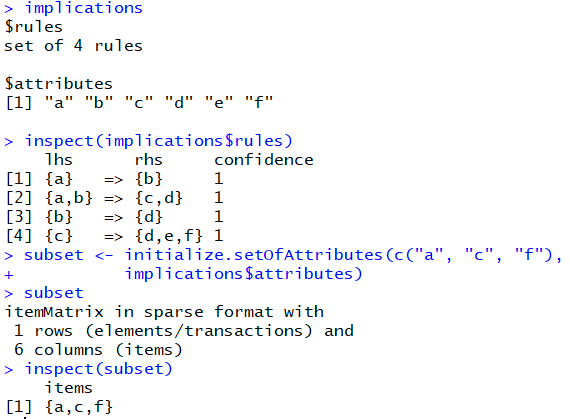
\includegraphics{InicializarConj}
        \caption{Ejemplo de inicializar conjunto de atributos}
        \label{fig:InicializarConj}
    \end{figure}

    En la variable implications se tiene un conjunto de 4 reglas y el conjunto de atributos que las componen.
    Al usar la funci\'on descrita en este punto, pas\'andole un subconjunto de todos los atributos, en este caso \{a,c,f\}, y 
    el conjunto total de los atributos, nos devuelve un itemMatrix. 
    
    Dicho itemMatrix est\'a compuesto s\'olo por esos tres atributos, aunque va a contener la informaci\'on de todos los que 
    componen las reglas; ya que deben estar para poder usar algunas funciones como uni\'on o intersecci\'on.



%%% is.singleton %%%
\subsubsection{Conjunto unitario}

    \textbf{Descripci\'on}
    
    Un conjunto unitario es aquel que tiene un s\'olo elemento. Por lo que esta funci\'on 
    devolver\'a TRUE si la longitud del conjunto que se le pase es igual a 1, o FALSE en caso 
    contrario.

    Esta es una funci\'on a la que se le puede pasar por par\'ametro una lista, un vector, 
    un conjunto de reglas o cualquier otro conjunto de elementos al que se le pueda aplicar la funci\'on 
    length().
    \\


    \textbf{C\'odigo}

    \lstinputlisting{r_code/basicLibrary/is.singleton.R}
    \bigskip

    \textbf{Ejemplo}

    En este caso, se van a proponer tres ejemplos diferentes para poder entender el comportamiento de esta funci\'on:

    \begin{figure}[H]
        \centering
        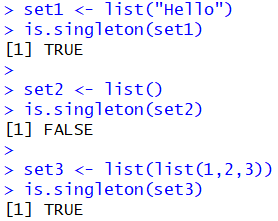
\includegraphics{singleton}
        \caption{Ejemplos de conjuntos unitarios}
        \label{fig:singleton}
    \end{figure}

    En el primer ejemplo, se puede observar que el conjunto es unitario porque est\'a compuesto por una sola cadena de caracteres. 
    Es decir, no cuenta caracter a caracter, sino la cadena, luego est\'a formado por un solo elemento y el resultado es TRUE.

    En el segundo ejemplo, tenemos una lista vac\'ia, por lo que como no tiene ning\'un elemento, el resultado es FALSE porque no es unitario.

    Por \'ultimo, se tiene una lista que contiene a otra lista con tres elementos dentro de ella. En este caso, se podr\'ia pensar que 
    no es unitario al ver los tres elementos, pero no, ya que el elemento que estamos estudiando es el primero, y este contiene solo una lista 
    en \'el, por lo que el resultado es TRUE, ya que s\'i es unitario.



%%% union.sets %%% 
\subsubsection{Uni\'on}

    \textbf{Descripci\'on}

    La uni\'on de dos conjuntos es una operaci\'on que devolver\'a otro conjunto formado por 
    todos los elementos de los dos conjuntos iniciales. Si un elemento se encuentra en los dos 
    conjuntos, s\'olo aparecer\'a una vez en el resultante.

    \[
    A \cup B = \{x\in U ~ | ~ x\in A ~ o ~ x\in B \}
    \]

    Esta funci\'on se usar\'a para la uni\'on de elementos de la clase itemMatrix, ya que lo que 
    se usa es itemUnion, una funci\'on perteneciente al paquete arules.
    \\


    \textbf{C\'odigo}

    \lstinputlisting{r_code/basicLibrary/union.sets.R}
    \clearpage

    \textbf{Ejemplo}

    \begin{figure}[H]
        \centering
        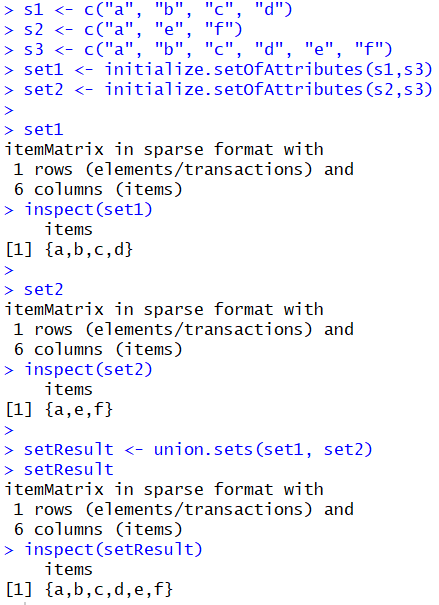
\includegraphics{union}
        \caption{Ejemplo de uni\'on de conjuntos}
        \label{fig:union}
    \end{figure}

    A continuaci\'on se va a explicar el anterior ejemplo paso a paso, ya que en \'el se han realizado varios pasos.

    Primero, se ha comenzado declarando tres vectores diferentes. Los dos primeros van a ser los dos conjuntos a unir, y el 
    tercero es la uni\'on de todas las variables. Despu\'es, se utiliza la funci\'on explicada anteriormente para convertir ambos 
    vectores en itemMatrix.

    Segundo, se observa que ambos conjuntos son de la estructura itemMatrix, con el mismo n\'umero de columnas. Esto es algo muy 
    importante, y por eso se ha usado la funci\'on initialize.setOfAttributes, ya que para utilizar la uni\'on, los elementos deben 
    estar en los dos conjuntos como informaci\'on, tal y como se vi\'o en la estructura de datos itemMatrix.

    Por \'ultimo, se realiza la uni\'on e inspeccionamos la variable resultante, y se comprueba que se ha realizado correctamente.



%%% intersection.sets %%% 
\subsubsection{Intersecci\'on}

    \textbf{Descripci\'on}
    
    La intersecci\'on de dos conjuntos A y B devolver\'a otro conjunto resultante U con los elementos 
    que se encuentren en ambos conjuntos iniciales. Es decir, el conjunto U estar\'a formado por los elementos 
    que est\'en tanto en A como en B.

    \[
        A \cap B = \{x\in U ~ | ~ x\in A ~ y ~ x\in B \}
    \]

    En este caso, tambi\'en se usar\'a con la estructura de datos itemMatrix que es la usada mayoritariamente con implicaciones 
    como ya se ha especificado antes.
    \\


    \textbf{C\'odigo}

    \lstinputlisting{r_code/basicLibrary/intersection.sets.R}
    \bigskip

    \textbf{Ejemplo}

    Para el ejemplo de esta funci\'on se van a utilizar los mismos conjuntos del ejemplo de la anterior funci\'on:

    \begin{figure}[H]
        \centering
        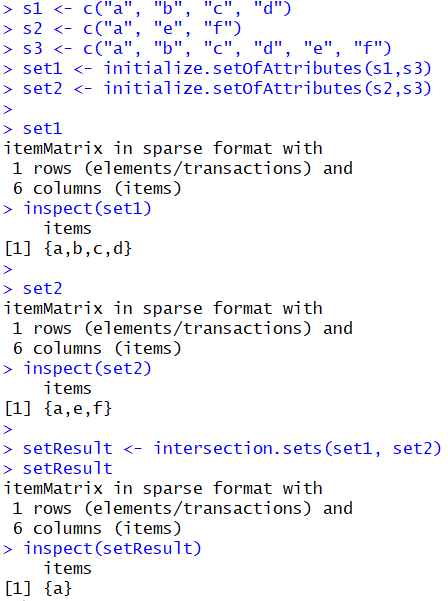
\includegraphics{interseccion}
        \caption{Ejemplo de intersecci\'on de conjuntos}
        \label{fig:interseccion}
    \end{figure}

    Para comenzar el ejemplo, se han realizado los mismos pasos que en el anterior, se declaran las variables y se convierten a 
    itemMatrix. 
    Por \'ultimo, se realiza la intersecci\'on de ambos conjuntos y vemos como el resultado es \'unicamente del elemento que se encuentra 
    en ambos conjuntos.

    \clearpage

%%% difference.sets %%% 
\subsubsection{Diferencia}

    \textbf{Descripci\'on}

    La diferencia de dos conjuntos da como resultado otro conjunto con los elementos que resultan de 
    eliminar a los elementos que forman el primer conjunto, los del segundo. Es decir, se obtendr\'ian 
    todos elementos del primer conjunto que no est\'an en el segundo.

    \[
        A - B = \{x\in A ~ y ~ x\notin B \}
    \]

    De nuevo, en nuestra funci\'on se usa una del paquete arules para poder utilizar la gran mayor\'ia de estructuras 
    que sean compatibles con restar elementos.
    \\


    \textbf{C\'odigo}

    \lstinputlisting{r_code/basicLibrary/difference.sets.R}
    \bigskip

    \textbf{Ejemplo}

    Para ilustrar bien esta funci\'on, vamos a volver a utilizar los conjuntos usados en la uni\'on e intersecci\'on para comprobar 
    cu\'al ser\'ia el resultado al realizar la diferencia de estos conjuntos.

    \begin{figure}[H]
        \centering
        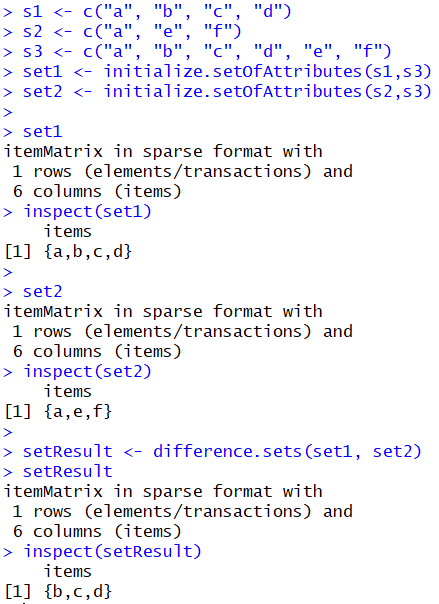
\includegraphics{diferencia}
        \caption{Ejemplo de diferencia de conjuntos}
        \label{fig:diferencia}
    \end{figure}

    En este caso, se vuelve a realizar todo de la mismo forma que en los anteriores casos, pero usamos la funci\'on difference.sets, y 
    con ella obtenemos como resultado un nuevo conjunto, en el que se encuentran los elementos del primer conjunto, eliminando los que 
    tambi\'en est\'en en el segundo.
    \clearpage


%%% is.included %%% 
\subsubsection{Inclusi\'on}

    \textbf{Descripci\'on}

    Un conjunto A est\'a incluido en un conjunto B, si A es subconjunto de B. Por lo que esta funci\'on 
    devolver\'a TRUE si cumple dicha propiedad, o FALSE en caso contrario.

    \[
        A \subseteq B ~ | ~  \forall ~ x \in A \to x \in B 
    \]

    De nuevo, esta funci\'on se utilizar\'a con elementos de la clase itemMatrix.
    \\

    \textbf{C\'odigo}

    \lstinputlisting{r_code/basicLibrary/is.included.R}
    \bigskip

    \textbf{Ejemplo}

    \begin{figure}[H]
        \centering
        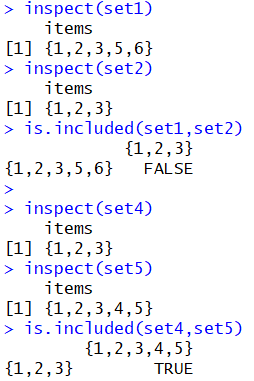
\includegraphics{inclusion}
        \caption{Ejemplos de inclusi\'on de conjuntos}
        \label{fig:inclusion}
    \end{figure}

    En este caso, se van a proponer dos ejemplos:

    En el primero no se cumple que el set1 est\'e incluido en el set2, aunque s\'i se cumplir\'ia al contrario, pero la inclusi\'on no es 
    una funci\'on que cumpla la propiedad sim\'etrica, luego en este caso el resultado es FALSE.

    En el segundo ejemplo s\'i que se cumple que el primer conjunto est\'e incluido en el segundo. Como se puede observar da igual el orden 
    en el que est\'en los elementos.



%%% is.empty.set %%% 
\subsubsection{Vac\'io}

    \textbf{Descripci\'on}

    Un conjunto es vac\'io si no contiene ning\'un elemento. Es decir, si el tama\~no del conjunto es 0, 
    podemos decir que est\'a vac\'io. 

    \[
        A = \{ \} = \emptyset
    \]

    \textbf{C\'odigo}

    \lstinputlisting{r_code/basicLibrary/is.empty.set.R}
    \bigskip

    \textbf{Ejemplo}

    \begin{figure}[H]
        \centering
        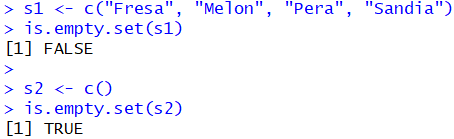
\includegraphics{vacio}
        \caption{Ejemplos de conjuntos vac\'ios}
        \label{fig:vacio}
    \end{figure}

    En el primer ejemplo, se puede ver que la funci\'on devuelve FALSE porque el conjunto contiene elementos.

    En cambio, en el segundo, el vector no contiene elementos, por lo que la funci\'on devuelve TRUE porque el conjunto no tiene 
    elementos.



    %%% equals.sets %%% 
\subsubsection{Igualdad}

    \textbf{Descripci\'on}

    Dos conjuntos A y B son iguales si su longitud es la misma, y si para cada elemento de A, existe uno igual 
    en B y para cada elemento de B existe uno igual en A.

    Ya que, seg\'un el axioma de extensionalidad:

    \[
        \forall A, B : \forall x, (x \in A \Leftrightarrow x \in B) \to A = B
    \]


    \textbf{C\'odigo}

    \lstinputlisting{r_code/basicLibrary/equals.sets.R}
    \bigskip

    \textbf{Ejemplo}

    \begin{figure}[H]
        \centering
        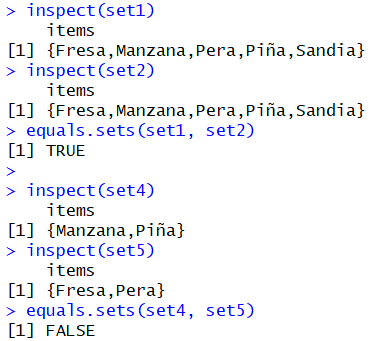
\includegraphics{igualdad}
        \caption{Ejemplos de igualdad de conjuntos}
        \label{fig:igualdad}
    \end{figure}

    De nuevo, se plantean dos ejemplos. En el primero, el resultado es TRUE, ya que visualmente se puede comprobar que ambos conjuntos son 
    iguales.

    En el segundo caso, la funci\'on devuelve FALSE porque los conjuntos no son iguales.



%%%%%%%%%%%%%%%%%%%%%%%%%%%%%%%%%%%%%%%%%%%%%%%%%%%%%%%%%%%%%%%%%%%%%%%%%%%%%%%%%%%%%%%%%%%%%%%%%%%%%%%%%%%%%%%%%%%%%%%%



%%% remove.imp %%% 
\subsubsection{Eliminar implicaci\'on}

    \textbf{Descripci\'on}

    Una de las tareas m\'as importantes de este TFG es trabajar con implicaciones. Una de las operaciones m\'as habituales 
    va a ser la de eliminar una implicaci\'on de un conjunto. Para ello, se ha definido la siguiente funci\'on, pas\'andole 
    como par\'ametros el conjunto de implicaciones y la posici\'on de la que se desea eliminar, devolver\'a un conjunto sin 
    dicha implicaci\'on.
    \\


    \textbf{C\'odigo}

    \lstinputlisting{r_code/basicLibrary/remove.imp.R}
    \bigskip

    \textbf{Ejemplo}

    \begin{figure}[H]
        \centering
        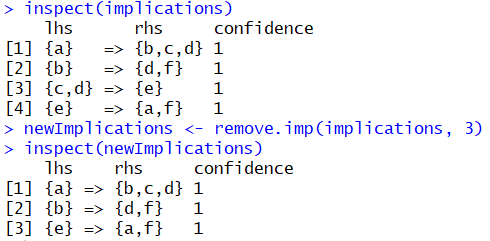
\includegraphics{removeImp}
        \caption{Ejemplo de eliminar implicaci\'on}
        \label{fig:removeImp}
    \end{figure}

    En este ejemplo, tenemos un conjunto inicial implications con cuatro implicaciones diferentes. A continuaci\'on se usa la 
    funci\'on remove.imp y con ella eliminamos la tercera.

    Finalizamos comprobando que efectivamente, en el nuevo conjunto solo se tienen tres implicaciones, quitando la tercera del conjunto 
    inicial.



%%% remove.all %%% 
\subsubsection{Vaciar conjunto}

    \textbf{Descripci\'on}

    Otra funci\'on que puede ser \'util es vaciar un conjunto. Se podr\'ia pensar que igualando el conjunto a nulo, 
    se podr\'ia obtener el resultado que se quiere conseguir. Pero no es as\'i, ya que lo que se quiere es un conjunto sin 
    elementos, pero que siga manteniendo su estructura de conjunto, no algo nulo. 
    
    Para ello, en esta funci\'on, vamos a devolver la posici\'on 0 del conjunto que se quiere vaciar. Recordemos, que en el 
    lenguaje R los arrays, listas y dem\'as estructuras de conjuntos comienzan en 1 y no en 0 como la gran mayor\'ia de lenguajes.
    Por lo que al devolver esta posici\'on, el resultado que se obtiene es el conjunto que se le hab\'ia pasado, pero sin ning\'un 
    elemento.
    \\


    \textbf{C\'odigo}

    \lstinputlisting{r_code/basicLibrary/remove.all.R}
    \bigskip

    \textbf{Ejemplo}

    \begin{figure}[H]
        \centering
        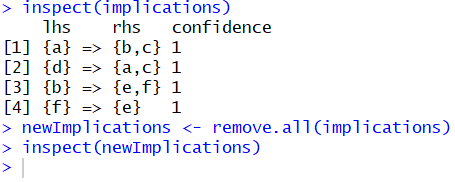
\includegraphics{removeAll}
        \caption{Ejemplo de vaciar conjunto}
        \label{fig:removeAll}
    \end{figure}

    En este caso, tenemos un conjunto de implicaciones, y si vaciamos dicho conjunto, el resultado es vac\'io ya que el nuevo 
    conjunto resultante no contiene ninguna implcaci\'on.



%%% add.imp %%% 
\subsubsection{A\~nadir implicaci\'on}

    \textbf{Descripci\'on}

    Igual que se puede querer eliminar una implicaci\'on, tambi\'en ser\'a posible a\~nadir una nueva. Por lo que esta funci\'on, 
    inserta la nueva implicaci\'on en la \'ultima posici\'on del conjunto. Como par\'ametros necesita el conjunto que se quiere ampliar, 
    el antecedente de la nueva implicaci\'on y el consecuente.

    As\'i que, se crea la nueva implicaci\'on, con las dos partes que se le pasan como par\'ametros, y se le concatena al conjunto 
    inicial para devolver un conjunto ampliado con una nueva implicaci\'on.
    \\


    \textbf{C\'odigo}

    \lstinputlisting{r_code/basicLibrary/add.imp.R}
    \bigskip

    \textbf{Ejemplo}

    \begin{figure}[H]
        \centering
        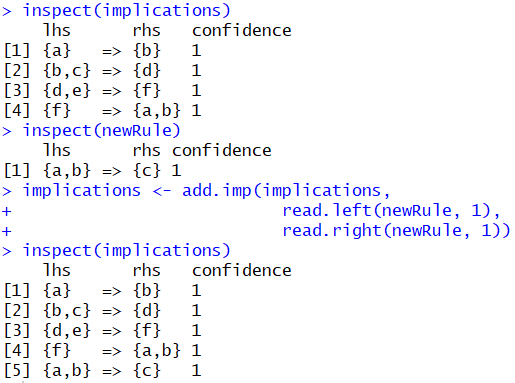
\includegraphics{addImp}
        \caption{Ejemplo de a\~nadir implicaci\'on}
        \label{fig:addImp}
    \end{figure}

    En este ejemplo tenemos un conjunto de 4 implicaciones en la variable implications, en newRule tenemos una \'unica regla que va 
    a ser la nueva a insertar. 

    Usando la funci\'on add.imp a\~nadimos la nueva regla como se puede observar en el nuevo conjunto implications.



%%% new.imp %%% 
\subsubsection{Nueva implicaci\'on}

    \textbf{Descripci\'on}

    Con esta funci\'on, vamos a insertar una nueva implicaci\'on, al igual que en el punto anterior, pero esta vez 
    de una forma un poco m\'as compleja. Ya que, en este caso, se van a realizar varias comprobaciones.

    Para cada implicaci\'on perteneciente al conjunto, se va a comprobar si el antecedente es igual al que se quiere insertar.
    En caso negativo, se continuar\'a con la siguiente implicaci\'on; y en caso afirmativo, se comprobar\'a si los consecuentes son 
    iguales. En caso de que se cumplan ambas afirmaciones, quiere decir que la implicaci\'on que intentamos insertar en el conjunto, 
    ya se encuentra en \'el, por lo que se devolver\'a el conjunto inicial sin ning\'un cambio.

    En el caso de que los antecedentes sean iguales, y los consecuentes no, se sustituir\'a esa regla por una nueva, en la que el antecedente 
    queda igual, y el consecuente estar\'a formado por la uni\'on del que ya estaba en el conjunto, y el nuevo que se quiere insertar. Y con 
    esto, se devolver\'ia el nuevo conjunto.

    El \'ultimo caso que se podr\'ia dar, es aquel en el que ninguna implicaci\'on del conjunto tenga el mismo antecedente que el que se 
    quiere insertar, por lo que al finalizar la iteraci\'on por todo el conjunto, se insertar\'ia la nueva regla y devolver\'ia el conjunto 
    resultante.
    \\

    \clearpage

    \textbf{C\'odigo}

    \lstinputlisting{r_code/basicLibrary/new.imp.R}
    \bigskip

    \textbf{Ejemplo}


    \begin{figure}[H]
        \centering
        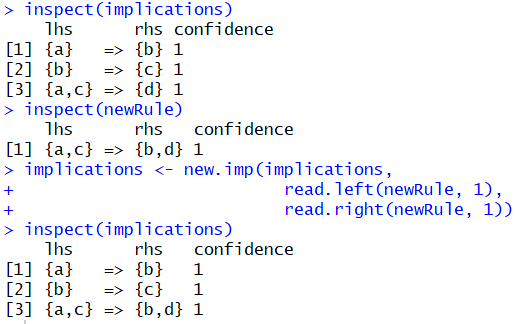
\includegraphics{newImp}
        \caption{Ejemplo de a\~nadir implicaci\'on}
        \label{fig:newImp}
    \end{figure}

    Aunque con esta funci\'on se podr\'ian realizar varios ejemplos seg\'un la implicaci\'on que se quiera a\~nadir, en este caso se 
    va a insertar una nueva en la que el antecedente ya se encuentra en el conjunto y el consecuente es nuevo.

    En la variable implications tenemos un conjunto de tres implicaciones, y en newRule, est\'a la nueva a insertar. Como se puede 
    observar, el antecedente de la nueva es igual al de la tercera implicaci\'on del conjunto. Se realiza la operaci\'on de a\~nadir 
    y vemos como en el conjunto resultante ha cambiado el consecuente de la \'ultima implicaci\'on tal y como se esperaba.



%%% read.left %%% 
\subsubsection{Leer antecedente}

    \textbf{Descripci\'on}

    Otra de las funciones b\'asicas a la hora de trabajar con implicaciones es poder obtener el antecedente de una determinada 
    implicaci\'on. Para ello, pas\'andole a esta funci\'on el conjunto que contiene a la implicaci\'on que queremos obtener, y su 
    posici\'on, nos devolver\'a el antecedente deseado.
    \\


    \textbf{C\'odigo}

    \lstinputlisting{r_code/basicLibrary/read.left.R}
    \bigskip

    \textbf{Ejemplo}

    Aunque esta funci\'on ya se ha utilizado en algunos ejemplos anteriores, veamos su resultado.

    \begin{figure}[H]
        \centering
        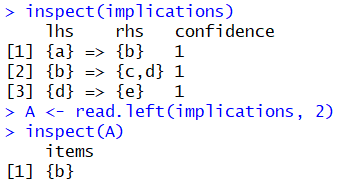
\includegraphics{readL}
        \caption{Ejemplo de leer antecedente}
        \label{fig:readL}
    \end{figure}

    Luego, en este ejemplo, tenemos un conjunto de tres implicaciones y con esta funci\'on leemos, en este caso, el antecedente de 
    la segunda implicaci\'on. 



%%% read.right %%% 
\subsubsection{Leer consecuente}

    \textbf{Descripci\'on}
    
    De igual forma que en el anterior punto, se puede querer obtener el consecuente de una implicaci\'on, luego, con el conjunto de 
    implicaciones y su posici\'on, esta funci\'on devolver\'a el consecuente de dicha implicaci\'on.
    \\


    \textbf{C\'odigo}

    \lstinputlisting{r_code/basicLibrary/read.right.R}
    \bigskip

    \textbf{Ejemplo}

    Al igual que en el anterior punto, esta funci\'on ya se ha usado en ejemplos anteriores, pero observemos cual es su resultado.

    \begin{figure}[H]
        \centering
        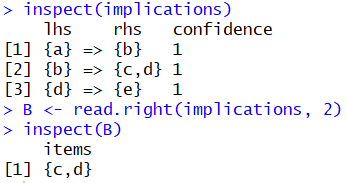
\includegraphics{readR}
        \caption{Ejemplo de leer consecuente}
        \label{fig:readR}
    \end{figure}

    Para este ejemplo, se ha usado el mismo conjunto de implicaciones que en el anterior, y leemos el consecuente de la misma 
    implicaci\'on que en el punto anterior.

    \clearpage

%%% substitute.imp %%% 
\subsubsection{Sustituir implicaci\'on}

    \textbf{Descripci\'on}

    La sustituci\'on de una implicaci\'on es una operaci\'on bastante \'util, ya que cuando se quieren unir dos implicaciones, puede que 
    se quiera que la nueva permanezca en un lugar determinado, para ello, esta funci\'on inserta la nueva implicaci\'on en el lugar que 
    se le indique. Como par\'ametros, necesita el conjunto de implicaciones, la posici\'on a cambiar, y los nuevos antedecente y consecuente.
    Para la utilizaci\'on de esta funci\'on se debe llamar a sustitute.imp, aunque esta, a su vez har\'a uso de add.imp.k, cuyos codigos se 
    muestran a continuaci\'on. 
    \\


    \textbf{C\'odigo}

    \lstinputlisting{r_code/basicLibrary/add.imp.k.R}

    \lstinputlisting{r_code/basicLibrary/substitute.imp.R}
    \bigskip

    \textbf{Ejemplo}

    \begin{figure}[H]
        \centering
        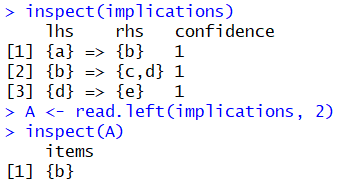
\includegraphics{readL}
        \caption{Ejemplo de leer antecedente}
        \label{fig:readL}
    \end{figure}

    Comenzamos con un conjunto de tres implicaciones en la variable implications, en newRule se tiene la implicaci\'on que se va 
    a insertar en el conjunto. Realizamos la operaci\'on de sustituir, en este caso la segunda implicaci\'on del conjunto, por la nueva. 
    Tal y como se observa en el conjunto resultante, se ha sustituido la anterior, por la nueva, tal y como se esperaba.


%%% included.left %%% 
\subsubsection{Incluido en antecedente}

    \textbf{Descripci\'on}

    Si tenemos dos implicaciones A y B y se quiere comprobar si el antecedente de A est\'a incluido en el de B, se debe usar 
    esta funci\'on. Le pasamos como par\'ametros un conjunto de implicaciones, y dos posiciones de dicho conjunto. Se usar\'an 
    las funciones is.included y read.left para comprobar si un antecedente est\'a incluido en otro, devolver\'a TRUE en caso 
    afirmativo, y FALSE en el contrario.
    \\


    \textbf{C\'odigo}

    \lstinputlisting{r_code/basicLibrary/included.left.R}
    \bigskip

    \textbf{Ejemplo}

    \begin{figure}[H]
        \centering
        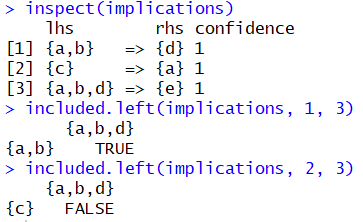
\includegraphics{incluidoL}
        \caption{Ejemplo de leer antecedente}
        \label{fig:incluidoL}
    \end{figure}

    Para este ejemplo tenemos un conjunto con tres implicaciones. Primero se comprueba si el antecedente de la primera implicaci\'on 
    est\'a incluido en el de la segunda, el resultado obtenido es TRUE, ya que se cumple la inclusi\'on.

    En cambio, en el segundo caso, se prueba el consecuente de la segunda, con el de la tercera, y como no se cumple, el resultado es FALSE.



%%% delete.set.of.IS %%% 
\subsubsection{Eliminar implicaciones con consecuente vac\'io}

    \textbf{Descripci\'on}

    Si se tiene un conjunto de implicaciones y alguna de ellas tiene su consecuente vac\'io, esta implicaci\'on no va a 
    aportar ning\'un tipo de conocimiento a este conjunto, por lo que se deben eliminar. Para ello, se usar\'ia esta funci\'on, 
    la cual, pas\'andole como par\'ametro dicho conjunto, nos devolver\'a uno nuevo eliminando las implicaciones con su consecuente 
    vac\'io.
    \\


    \textbf{C\'odigo}

    \lstinputlisting{r_code/basicLibrary/delete.set.of.IS.R}
    \bigskip

    \textbf{Ejemplo}

    \begin{figure}[H]
        \centering
        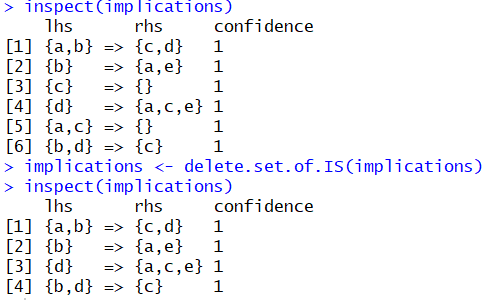
\includegraphics{deleteIS}
        \caption{Ejemplo de eliminar implicaciones con consecuente vac\'io}
        \label{fig:deleteIS}
    \end{figure}

    Comenzamos con un conjunto de seis implicaciones, en el que dos de ellas tienen su consecuente vac\'io. Al realizar la 
    operaci\'on de borrar los consecuentes vacios, obtenemos un nuevo conjunto con cuatro implicaciones, ya que las que ten\'ian 
    sus consecuentes sin elementos, han sido eliminadas.



%%% size.set %%% 
\subsubsection{Tama\~no del conjunto}

    \textbf{Descripci\'on}

    Por tama\~no del conjunto, se entiende el n\'umero de elementos, repetidos o no, que lo componen. 
    Es decir, para calcular el tama\~no de un conjunto, se va a realizar la suma de los tama\~nos de cada una de 
    las implicaciones que forman el conjunto.
    \\


    \textbf{C\'odigo}

    \lstinputlisting{r_code/basicLibrary/size.set.R}
    \bigskip

    \textbf{Ejemplo}

    \begin{figure}[H]
        \centering
        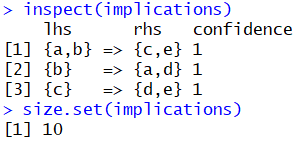
\includegraphics{size}
        \caption{Ejemplo de tama\~no de conjunto}
        \label{fig:size}
    \end{figure}

    En este ejemplo se tiene un conjunto con tres implicaciones, su tama\~no, tal y como muestra el ejemplo es de 10. 
    Este resultado viene de sumar cu\'antos elementos tiene cada implicaci\'on, en este caso:
    \[
        4 + 3 + 3 = 10    
    \]



%%% cadinality.set %%% 
\subsubsection{Cardinalidad del conjunto}

    \textbf{Descripci\'on}

    La cardinalidad de un conjunto, se entiende como el n\'umero de implicaciones que lo componen. Es decir, lo que 
    tambi\'en se suele denominar como longitud del conjunto.
    \\


    \textbf{C\'odigo}

    \lstinputlisting{r_code/basicLibrary/cardinality.set.R}
    \bigskip

    \textbf{Ejemplo}


    \begin{figure}[H]
        \centering
        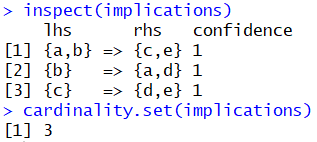
\includegraphics{cardinality}
        \caption{Ejemplo de cardinalidad de conjunto}
        \label{fig:cardinality}
    \end{figure}

    La cardinalidad, tal y como se ha explicado arriba es el n\'umero de implicaciones que tiene un conjunto, por lo que como 
    se puede observar en este ejemplo, como tiene tres implicaciones, su cardinalidad es tres.



%%% core %%% 
\subsubsection{Core}

    \textbf{Descripci\'on}

    A esta funci\'on se le pasa un conjunto de atributos Omega, junto con un conjunto de implicaciones Gamma. 
    Devolver\'a un conjunto de datos resultante de eliminar de Omega todos los atributos que se encuentren en los 
    consecuentes de las implicaciones que forman Gamma. 

    \[
        core(\Omega , \Gamma ) = \Omega ~ \textbackslash ~ ( \bigcup_{A \to B \in \Gamma} B )    
    \]
    
    Esta no es precisamente una funci\'on b\'asica, pero se ha incluido en este apartado, ya que se utilizar\'a 
    en el algoritmo de claves minimales realizado en el segundo tomo de este TFG.
    \\


    \textbf{C\'odigo}

    \lstinputlisting{r_code/basicLibrary/core.R}
    \bigskip

    \textbf{Ejemplo}


    \begin{figure}[H]
        \centering
        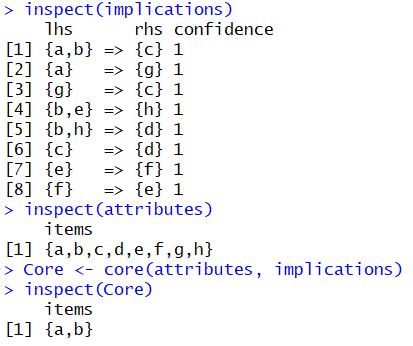
\includegraphics{core}
        \caption{Ejemplo de core de un conjunto}
        \label{fig:core}
    \end{figure}

    En el ejemplo, tenemos como punto de partida un conjunto con cinco implicaciones y todos los elementos de ese conjunto en 
    un itemMatrix. Realizamos la operaci\'on core y se obtiene como resultado un itemMatrix con dos de los elementos de las implicaciones. 
    Tal y como se ha explicado anteriormente, este resultado se obtiene de restar de todos los atributos, los que est\'an en los consecuentes 
    de las implicaciones.



%%% body %%% 
\subsubsection{Body}

    \textbf{Descripci\'on}

    Al igual que en el punto anterior, esta funci\'on se utilizar\'a en el algoritmo para calcular claves minimales, aunque junto con 
    el anterior, se han incluido aqu\'i.

    Siendo Omega un conjunto de atributos, y Gamma un conjunto de implicaciones, se define la funci\'on body como la diferencia 
    de la uni\'on de los antecedentes de Gamma, menos el cierre del core de Omega y Gamma. 

    \[
        body(\Omega , \Gamma ) = ( \bigcup_{A \to B \in \Gamma} B ) ~ \textbackslash ~ core(\Omega , \Gamma )^+
    \]

    \textbf{C\'odigo}

    \lstinputlisting{r_code/basicLibrary/body.R}
    \clearpage

    \textbf{Ejemplo}


    \begin{figure}[H]
        \centering
        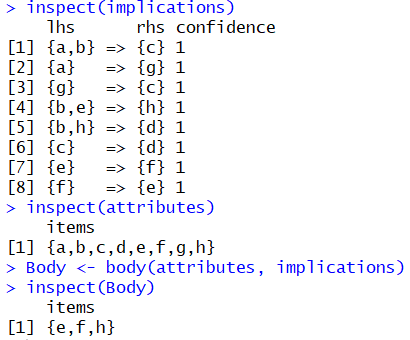
\includegraphics{body}
        \caption{Ejemplo de body de un conjunto}
        \label{fig:body}
    \end{figure}

    Para este ejemplo, se usa el mismo conjunto de implicaciones que en el anterior punto. Sin embargo, el resultado en este caso es 
    el conjunto vac\'io, ya que es el resultado de restar de todos los elementos que se encuentran en los antecedentes de las implicaciones, 
    el resultado de el cierre del core de Omega y Gamma.

    
\clearpage

\section{Generadores aleatorios}

\subsection{Sistemas de implicaciones aleatorios}

    \textbf{Introducci\'on}

    Cuando se quieren realizar pruebas con un algoritmo, se aconseja utilizar conjuntos generados de forma aleatoria, para que, por ejemplo, 
    en los an\'alisis de tiempo, los resultados no sean influidos por dichos conjuntos. Actualmente, hasta donde se conoce, no existe un 
    generador aleatorio de sistemas de implicaciones en ninguna de las diferentes \'areas, como pueden ser data mining, machine learning, 
    IA, sistemas inteligentes, redes neuronales...

    Luego, debido a esto, se ha decidido realizar una funci\'on que pueda ser usada para este fin y ponerla a disposici\'on de toda la comunidad 
    junto a este paquete.
    \\ 


    \textbf{Descripci\'on}
    
    Esta funci\'on va a generar uno o m\'as sistemas de implicaciones siguiendo una serie de par\'ametros que se pueden elegir a la 
    hora de ejecutar dicha funci\'on para obtener el conjunto como sea m\'as adecuado a lo que se desee hacer.

    Los atributos de las implicaciones van a ser del tipo a0, a1... Comenzando en 0, de forma consecutiva hasta el n\'umero que sea 
    necesario para tener todos los atributos que el usuario quiera. Los par\'ametros de esta funci\'on son:

    \begin{itemize}
        \item \textbf{numAttributes:}

        Aqu\'i se debe especificar cu\'antos atributos diferentes se quiere que tengan las implicaciones que se van a generar. Es un 
        par\'ametro obligatorio para la utilizaci\'on de esta funci\'on. Como se ha comentado anteriormente, los atributos ser\'an de la 
        forma a0, a1, a2... El valor de este par\'ametro debe ser mayor que 0.

        \clearpage

        \item \textbf{numDependencies:}

        Otro par\'ametro obligatorio es el n\'umero de dependencias que se quieren obtener, si se elige obtener m\'as de un archivo 
        con diferentes sistemas de implicaciones, como se ver\'a m\'as adelante, cada uno de dichos ficheros incluir\'a el n\'umero 
        de implicaciones que se le indique aqu\'i. Por supuesto, el valor de este par\'ametro tambi\'en debe ser mayor que 0.

        
        \item \textbf{difference:}

        Este par\'ametro opcional indica el n\'umero m\'aximo de diferencia de elementos entre el antecedente y el consecuente. Se puede 
        insertar un n\'umero negativo, lo que indicar\'a que se desea que haya m\'as atributos en el consecuente. Por lo que, si el n\'umero 
        es positivo, el antecedente tendr\'a m\'as atributos.

        En este caso, hay que tener en cuenta que el valor absoluto del n\'umero insertado en este par\'ametro, debe ser menor 
        que el n\'umero total de atributos.

        En caso de no especificar nada, la diferencia de atributos entre antecedente y consecuente ser\'a aleatoria.


        \item \textbf{percentage:}

        Este par\'ametro es bastante parecido al anterior, solo que en este caso, se trata del m\'aximo porcentaje de diferencia entre 
        el antecedente y el consecuente. Al igual que en el anterior, si el porcentaje es negativo, el consecuente ser\'a mayor, y en caso de 
        ser positivo, el antecedente tendr\'a m\'as atributos que el consecuente. Al ser un porcentaje, el valor debe ser menor estricto que 
        100.

        Cabe especificar, que tanto este par\'ametro, como el anterior, se tratan de tama\~nos m\'aximos, es decir, que no todas las implicaciones 
        van a tener la diferencia exacta que se le especifique entre antecedente y consecuente, sino que el n\'umero o porcentaje ser\'a la 
        mayor diferencia que se encontrar\'a en el sistema de implicaciones.


        \item \textbf{maxLeftSize:}

        Con este par\'ametro opcional, se puede especificar el n\'umero de elementos m\'aximo que se quiere que tenga el antecedente, como 
        es de esperar, no debe superar al n\'umero total de atributos.


        \item \textbf{maxRightSize:}

        Junto con el anterior, podemos especificar, en este caso, el n\'umero de elementos m\'aximo del consecuente. Ambos son par\'ametros 
        opcionales, pero si el usuario decide especificar el tama\~no m\'aximo del antecedente, tambi\'en deber\'a hacer lo mismo con el 
        consecuente y viceversa.


        \item \textbf{nameExitFile:}

        Este se trata de un par\'ametro obligatorio, se le debe pasar una cadena de caracteres sin la extensi\'on del archivo, ya que 
        la funci\'on devolver\'a un archivo con extensi\'on .R.


        \item \textbf{numFiles:}

        Por \'ultimo, un par\'ametro opcional en el que se puede especificar cu\'antos ficheros se quiere que se generen. Si no se especifica, 
        solo se generar\'a un archivo, en caso contrario, los archivos tendr\'an como nombre el especificado seguido de un guion bajo y un n\'umero 
        para distinguirlos.

    \end{itemize}

    Hay que precisar, que algunos de los par\'ametros anteriores son excluyentes. Es decir, si se especifica el par\'ametro difference, tanto 
    percentage, como maxLeftSize y maxRightSize deben dejarse nulos. O si se especifica percentage, deber\'an quedar vac\'ios difference y 
    maxLeftSize y maxRightSize. 
    En cambio, maxLeftSize siempre debe ir acompa\~nado de maxRightSize y viceversa, aunque en caso de especificarlos, difference y percentage, 
    deben estar nulos.
    Los par\'ametros que siempre se le deben pasar a la funci\'on son: numAttributes, numDependencies y nameExitFile.

    Por \'ultimo, hay que especificar que el sistema o sistemas de implicaciones que se obtengan, no tendr\'an redundancias y se habr\'a aplicado 
    la funci\'on de composici\'on, por lo que al realizar todas estas operaciones, si el n\'umero de implicaciones que se quiere obtener es 
    alto, el tiempo que tardar\'a el algoritmo en obtener dicho sistema, tambi\'en ser\'a alto.
    \\

    \bigskip

    \textbf{C\'odigo}

    \lstinputlisting{r_code/randomGenerators/randomImp.R}
    \clearpage


    \textbf{Ejemplo}

    Como se ha visto anteriormente, este algoritmo se puede utilizar con muchas combinaciones diferentes dependiendo de los par\'ametros 
    que se utilicen. As\'i que, se van a proponer tres ejemplos diferentes de c\'omo usar esta funci\'on, aunque las posibilidades 
    son mucho mayores.

    \bigskip

    \begin{figure}[H]
        \centering
        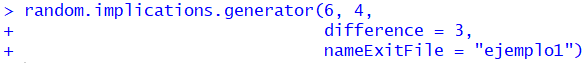
\includegraphics{randomImp1}
        \caption{Ejemplo 1 de sistemas de implicaciones aleatorios}
        \label{fig:randomImp1}
    \end{figure}

    En este primer ejemplo, se va a generar un sistema con cuatro implicaciones, utilizando 6 atributos diferentes, con una diferencia m\'axima 
    de 3 elementos entre el antecedente y el consecuente, siendo mayor el antecedente, como nombre del fichero se utilizar\'a ejemplo1.
    
    En dicho fichero se ha escrito lo siguiente:

    \begin{verbatim}
        a1 a3 a4 a6 -> a5 
        a1 a2 a4 a5 -> a6 
        a3 a6 -> a4 
        a1 a2 a6 -> a3    
    \end{verbatim}


    \begin{figure}[H]
        \centering
        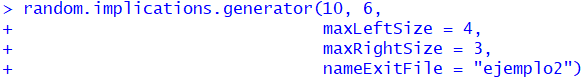
\includegraphics{randomImp2}
        \caption{Ejemplo 2 de sistemas de implicaciones aleatorios}
        \label{fig:randomImp2}
    \end{figure}

    En este segundo ejemplo se han generado con 10 atributos, 6 implicaciones, con un tama\~no m\'aximo de 4 para el antecedente y 3 para el 
    consecuente. El nombre del fichero de salida ser\'a ejemplo2.

    \begin{verbatim}
        a1 a10 a6 a7 -> a9 
        a5 -> a4 
        a10 a3 a6 a8 -> a9 
        a8 -> a9 
        a1 a10 a6 -> a7 
        a3 a7 a9 -> a4 
    \end{verbatim}
    Como se puede observar, la salida cumple todos los requisitos que le hemos puesto. En este caso, se observa que solo se han usado 9 de 
    los 10 atributos que se ped\'ian, ya que con la simplificaci\'on del conjunto, se ha llegado a perder el atributo a2.
    \\
    
    \bigskip

    Por \'ultimo, se ejecuta una tercera vez esta funci\'on para comprobar c\'omo es el error que se produce, en este caso, al pasarle vac\'io 
    el nombre del fichero de salida:

    \begin{figure}[H]
        \centering
        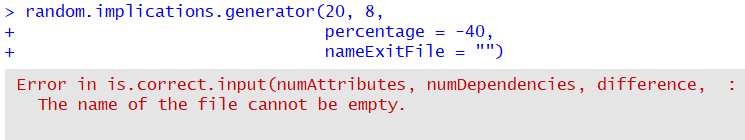
\includegraphics{randomImp3}
        \caption{Ejemplo 3 de sistemas de implicaciones aleatorios}
        \label{fig:randomImp3}
    \end{figure}

    \clearpage


\subsection{Contextos aleatorios}

    \textbf{Introducci\'on}

    En este caso, al igual que en el anterior, hasta donde se sabe, en la comunidad de FCA tampoco existe ning\'un generador aleatorio de 
    contextos, y son bastante necesarios para, como se ha nombrado antes, por ejemplo, realizar pruebas de los diferentes algoritmos.

    As\'i que, se decide realizar un algoritmo de este tipo para a\~nadirlo a este paquete para que toda persona interesada pueda 
    utilizarlo.
    

    \textbf{Descripci\'on}

    Un contexto formal \( (G, M, I) \) consiste en dos conjuntos, G y M, y una relaci\'on binaria \( I \subseteq G x M \). Los elementos 
    de G se llaman objetos, los de M, atributos de \( (G, M, I) \). Si \(g \in G ~ y ~ m \in M \) est\'an relacionados seg\'un I, se escribir\'a 
    \( (g,m) \in I ~ o ~ g I m \) y se leer\'a como ``el objeto g tiene el atributo m".

    \textcolor{red}{A\~nadir referencia paper}

    La manera habitual de representar un contexto formal es mediante una tabla, la cual contar\'a con una fila para cada objeto y una columna 
    para cada atributo, con una cruz en la intersecci\'on entre una fila g con una columna m sii el objeto g tiene un atributo m, \( (g,m) \in 
    I \).

    Por ello, la estructura m\'as sencilla a la hora de programar un algoritmo para contextos formales en R ser\'a un data.frame.
    \\


    Luego, en este caso, esta funci\'on va a generar un contexto formal siguiendo algunos par\'ametros que se pueden elegir a la 
    hora de ejecutar dicha funci\'on para obtener el contexto lo m\'as adecuado posible para lo que se desee.

    Los objetos del contexto se van a representar como obj1, obj2... y los atributos como att1, att2... Ambos comenzando en 1, de forma 
    consecutiva hasta el n\'umero que el usuario indique.
    \\

    Los par\'ametros de esta funci\'on son:

    \begin{itemize}
        \item \textbf{num.obj:}

        Con este par\'ametro obligatorio se indicar\'a el n\'umero de objetos que debe tener el contexto, o lo que es lo mismo, 
        cu\'antas filas tendr\'a el data.frame. Este par\'ametro debe ser mayor que uno, 
        ya que no tendr\'ia sentido crear un contexto sin objetos.


        \item \textbf{num.attr:}

        Este par\'ametro obligatorio indicar\'a cual ser\'a el n\'umero de atributos del contexto, es decir, las columnas que tendr\'a el 
        data.frame. De nuevo, debe ser un n\'umero mayor que uno, ya que tampoco tendr\'ia sentido en este caso crear un contexto sin 
        atributos.

        \item \textbf{sparness:}

        Como par\'ametro opcional, tenemos la dispersi\'on, es decir la probabilidad de que un objeto tenga un atributo, o lo que es 
        lo mismo a la hora de programarlo, que en el cruce de columna y fila, haya un uno.
        Como este par\'ametro se trata de una probabilidad, su valor debe estar entre 0 y 1.

    \end{itemize}


    Cuando se utilice la funci\'on, esta devolver\'a un data.frame, siendo los nombres de filas los objetos, y los de las columnas 
    los atributos.


    \bigskip

    \textbf{C\'odigo}

    A la hora de optimizar el c\'odigo, si el par\'ametro sparness no est\'a vac\'io, se ha decidido generar aleatoriamente el n\'umero de 
    TRUE o FALSE dependiendo de cu\'al de los dos sea menor. Es decir, si el usuario inserta en el par\'ametro sparness 0.2, con 4 objetos 
    y 5 atributos, esto querr\'a decir que debe haber cuatro TRUE entre los 20 elementos a generar aleatoriamente. Por lo que en este caso, 
    el n\'umero de TRUE ser\'a menor que el de FALSE, as\'i que se colocar\'an cuatro TRUE aleatoriamente, rellenando las dem\'as posiciones 
    del data.frame de FALSE.

    Como el algoritmo se va a ejecutar de formas diferentes dependiendo de las entradas que elija el usuario, se ha decidido modularizarlo 
    para poder comprenderlo bien. Veamos las diferentes partes:


    Aqu\'i tenemos el algoritmo principal, que ser\'a el que el usuario utilice:

    \lstinputlisting{r_code/randomGenerators/context.R}
    \bigskip

    En el caso de que el usuario no especifique el par\'ametro sparness, el contexto se generar\'a totalmente de forma aleatoria:

    \lstinputlisting{r_code/randomGenerators/noSpar.R}
    \clearpage

    Y como se ha especificado anteriormente, dependiendo de cu\'al sea la probabilidad de dispersi\'on elegida por el usuario, se generar\'an 
    los TRUE o los FALSE:

    \lstinputlisting{r_code/randomGenerators/ones.R}
    \bigskip
    \lstinputlisting{r_code/randomGenerators/zeros.R}
    \bigskip

    \textbf{Ejemplo}

    Como primer ejemplo, se va a generar un contexto sin el par\'ametro sparness, con 4 objetos y 5 atributos:

    \begin{figure}[H]
        \centering
        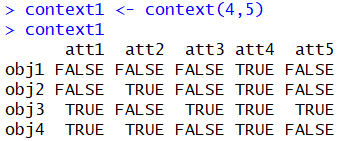
\includegraphics{randomC1}
        \caption{Ejemplo 1 de contextos aleatorios}
        \label{fig:randomC1}
    \end{figure}

    \bigskip
    Y como segundo ejemplo, un contexto con 6 objetos y 8 atributos, con 0.5 de sparness:

    \begin{figure}[H]
        \centering
        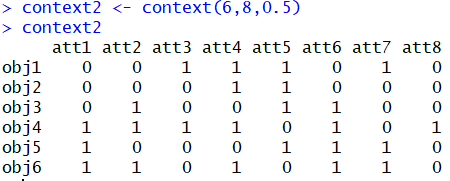
\includegraphics{randomC2}
        \caption{Ejemplo 2 de contextos aleatorios}
        \label{fig:randomC2}
    \end{figure}

    Como podemos observar, el n\'umero de FALSE y TRUE es el mismo, ya que se ha elegido como par\'ametro de esparness 0.5.
    
\clearpage

%Data mining
\subsection{Data mining}
\clearpage



\newpage
\thispagestyle{empty}
\mbox{}


\newpage
%\section{Paquetes}
\subsection{Introducci\'on}


El lenguaje R es un lenguaje que est\'a muy fundamentado en la comunidad, dispone de una gran comunidad que 
contribuye al desarrollo, mejora y extensi\'on de este lenguaje. La unidad fundamental a la hora de compartir 
nuestro trabajo con la comunidad es el paquete. Es por ello por lo cual se va a desarrollar un estudio sobre 
c\'omo crear un paquete en el lenguaje R y c\'omo distribuirlo de forma que este\'e disponible para toda la 
comunidad y contribuir al desarrollo de este lenguaje.
Para ello primero hablaremos del equipo CRAN, los encargados de mantener y revisar todos los paquetes que
se encuentran disponibles para este lenguaje en el principal repositorio del mismo, luego hablaremos de 
c\'omo se estructura un paquete, directorios y archivos principales que ha de contener el mismo. Por \'ultimo, 
se detallar\'a todo el proceso de creaci\'on, documentaci\'on y distribuci\'on del paquete, apoyado con 
consejos, buenas pr\'acticas y recomendaciones que har\'an m\'as f\'acil este proceso y dotar\'an a nuestro 
paquete de mayor facilidad de uso, distribuci\'on, posibles ampliaciones futuras y detecci\'on y correcci\'on 
de posibles fallos.
Como herramientas fundamentales para seguir este proceso, haremos uso del entorno de desarrollo R Studio, 
de la herramienta Rtools y de los paquetes de R, devtools y \textbf{roxygen2}.

\'a
\'e
\'i
\'o
\'u
\~n

\subsection{?`Qu\'e es CRAN?}

Es el principal repositorio de paquetes estables de R, del cual se descargar\'an la mayor\'ia de los paquetes 
necesarios para un proyecto.
CRAN se mantiene gracias al esfuerzo de los voluntarios \textbf{(El equipo CRAN)} y los recursos de la fundaci\'on R. 
Este equipo se encarga de ponerse en contacto con las personas que se encargan de mantener sus propios paquetes, 
en caso de que algo no vaya bien.
Tambi\'en, en casos excepcionales, pueden modificar algo de un paquete que haya fallado al actualizar la versi\'on 
de R.
Por \'ultimo, tambi\'en encontramos al \textbf{R Core Team}, un grupo formado por unas 20 personas que se dedica a modificar 
el c\'odigo fuente de R.

\subsection{Estructura de paquetes en R}

Un paquete (\textbf{package}) es una colecci\'on de funciones, datos y c\'odigo R que se almacenan en una carpeta 
conforme a una estructura bien definida y f\'acilmente accesible para R.
Estos paquetes sirven para incrementar la potencia de R mejorando su funcionalidad base, o a\~nadiendo 
nuevas. El directorio donde se almacenan los paquetes se llama libreri\'ia (\textbf{library}).
Como ya se ha comentado, R ya tiene instalados por defecto algunos paquetes, otros muchos est\'an disponibles 
para descargarlos e instalarlos. Una vez completados los dos pasos anteriores, los paquetes tienen que ser 
cargados en cada sesi\'on que se vayan a usar.

Es importante distinguir entre tener un paquete instalado en el ordenador y tenerlo cargado en memoria:

\begin{itemize}
    \item Tenerlo instalado en el ordenador significa simplemente que en alg\'un momento lo hemos bajado de internet 
y lo hemos copiado en alg\'un directorio en que R lo puede localizar.
    \item Tenerlo cargado en memoria significa que durante nuestra sesi\'on de trabajo R ha lei\'ido el contenido del 
paquete y ha incorporado las funciones que contiene a su espacio de trabajo, de tal forma que tales funciones 
pueden ya ser invocadas y ejecutadas.
\end{itemize}

Una vez que tenemos claro que\'i es un paquete en R, veamos su estructura, esto es, directorios y archivos 
m\'as importantes que lo componen.
Un paquete en R no est\'a compuesto s\'olo del c\'odigo en dicho lenguaje, sino que tambie\'in incorpora m\'as ficheros, 
los cuales se van a detallar a continuaci\'on.
La informaci\'on b\'asica sobre un paquete se proporciona en el archivo \textbf{\textbf{DESCRIPTION}}, donde podemos ver que\'i hace 
el paquete, quie\'in es el autor o autores, quie\'in realizar\'a el mantenimiento, a que\'i versi\'on pertenece la 
documentaci\'on... entre otros datos.
En el fichero \textbf{NAMESPACE} se deber\'an especificar todos aquellos objetos que ser\'an importados o exportados del paquete.
En \textbf{LICENSE}, se incluir\'a una copia de la licencia para informar al usuario.
Para finalizar con los ficheros, podremos encontrar en algunos casos uno llamado \textbf{NEWS}, en el cual estar\'an 
incluidos los cambios que se realizan de una versi\'on a otra.
La carpeta \textbf{R} es el n\'ucleo de la estructura, aqui\'i se encuentran todos los archivos \textbf{\textbf{.R}} con el c\'odigo de las 
funciones que incluya dicho paquete.
Es recomendable no aglutinar todo el c\'odigo en un mismo archivo sino separar las funciones que tienen relaci\'on 
o que cumplen cierta funcionalidad en archivos separados, asi\'i como dar un nombre descriptivo a los archivos.
La carpeta \textbf{man} contiene los ficheros de ayuda, es decir, estos paquetes compondr\'an el “Manual de referencia” 
del paquete. Cada uno de estos ficheros, se debe corresponder a cada uno de los archivos que se encuentran 
en la carpeta R, pero en este caso, su nombre sera \textbf{nombre\_del\_archivo\textbf{.R}d}.
En la carpeta data se encontrar\'an todos los ficheros de datos que se deseen incorporar al paquete. La extensi\'on 
de estos ficheros ser\'an \textbf{\textbf{.R}Data} o \textbf{\textbf{.R}da}.
Por \'ultimo, en la carpeta \textbf{inst} estar\'an todos aquellos ficheros que deseemos que se instalen con el paquete.


En caso de tener c\'odigo en otro lenguaje, adem\'as de R, los ficheros correspondientes se incluir\'an en la carpeta 
\textbf{src}.
De estos archivos se hablar\'a m\'as adelante en la secci\'on de documentaci\'on.


\subsection{Requisitos previos}

\begin{itemize}
    \item R Studio
    \item Paquete \textbf{devtools}
    \item Paquete \textbf{\textbf{roxygen2}} 
    \item Rtools
\end{itemize}

\subsection{Crear proyecto R}

Una vez que se tiene clara la estructura de los paquetes en R y cu\'ales son los archivos
imprescindibles que deber\'a tener nuestro paquete, podemos comenzar a trabajar en su
creaci\'on. Si bien es cierto que existen diferentes formas de crear y trabajar con los paquetes
en R, en este caso lo podemos hacer tanto con R Studio, como se muestra a continuaci\'on,
como con \textbf{devtools::create(}\enquote*{ruta/del/paquete/nombreDelPaquete}\textbf{)}, ambas opciones nos
proporcionaran un \enquote*{esqueleto} del paquete con los archivos imprescindibles.
Una vez abierto R Studio, lo primero que debemos hacer es crear un nuevo proyecto para
ellos vamos a: 
\begin{center}
    \textbf{file > new project > new directory > r package} 
\end{center}

En este momento deber\'iamos ver una ventana como la siguiente:

Figura 1

En la casilla \textbf{Package name:} especificamos el nombre de nuestro proyecto; en la casilla
\textbf{Create package based on source files} podemos a\~nadir (picando en el bot\'on \textbf{Add}) los
archivos \textbf{.R} que contengan nuestras funciones, si los hemos generado previamente (no es
estrictamente necesario a\~nadirlos ahora, se pueden a\~nadir posteriormente).
Por \'ultimo, indicamos el directorio ra\'iz en el que se situar\'a el subdirectorio en que estar\'an
contenidos los archivos de nuestro proyecto. Resulta conveniente disponer de una carpeta
espec\'ifica para paquetes de R. R Studio crear\'a un subdirectorio dentro de dicha carpeta con
el nombre de nuestro nuevo paquete.
Si se quiere llevar a cabo un control de versiones del paquete se puede hacer clic en \textbf{Create
a git repository}.
Al pinchar en el bot\'on \textbf{Create Project} se crear\'a un directorio en la ubicaci\'on indicada con la
estructura necesaria para que R pueda construir el paquete:

Figura 2



\subsection{Crear/a\~nadir las funciones que componen el paquete}

A continuaci\'on, debemos a\~nadir a la carpeta R los scripts/funciones que incluye nuestro
paquete.
Para que R pueda generar autom\'aticamente el archivo de ayuda para nuestras funciones
usando \textbf{roxygen2} incluimos las siguientes l\'ineas antes del comienzo de la funci\'on:

Figura 3

Para ello debemos configurar las \textbf{Build Tools} de nuestro proyecto:

Figura 4

Una vez ajustada la configuraci\'on, pinchamos en \textbf{Install and Restart} de la pesta\~na \textbf{Build},
esto har\'a que \textbf{roxygen2} genere autom\'aticamente el archivo \textbf{.Rd} de ayuda de nuestra funci\'on
en la carpeta \textbf{man}.\\
La documentaci\'on de ayuda de nuestras funciones se detallar\'a m\'as en la secci\'on de
documentaci\'on.

\subsection{Documentaci\'on}

La documentaci\'on es una de las partes m\'as importantes del paquete en R, esta sirve para
ayudar a los usuarios a usar el paquete, para los desarrolladores que quieran extenderlo e
incluso para el propio creador del paquete, para en un futuro poder recordar para que serv\'ian
sus funciones.
Por ello, a continuaci\'on, se proceder\'a a describir los archivos m\'as importantes de
documentaci\'on que todo paquete de R debe contener.

\subsubsection{Archivo DESCRIPTION}

Uno de los archivos m\'as importantes dentro de la estructura de un paquete en R es el archivo
\textbf{DESCRIPTION}, su funci\'on es la de almacenar todos los metadatos relacionados con el
paquete al que pertenece, como pueden ser el autor o la licencia bajo la que se distribuye el
paquete.
En primer lugar, el archivo \textbf{DESCRIPTION} es lo que indica a R Studio que el directorio que lo
contiene es un paquete. Cuando creamos un proyecto e indicamos a R Studio que se va a
tratar de un paquete, este autom\'aticamente genera una plantilla del archivo \textbf{DESCRIPTION}
con los campos m\'inimamente necesarios.

Figura 5

De igual forma, si creamos el paquete haciendo uso de la herramienta \textbf{devtools}, obtendremos
una plantilla similar.

Figura 6

Este archivo usa un formato simple denominado Debian control format (DCF) cuya estructura
es muy simple, cada l\'inea consiste en un campo y un valor separados por \enquote*{:}, cuando el valor
8ocupa m\'as de una l\'inea hay que tabular las l\'ineas, como se puede ver en el campo
\textbf{DESCRIPTION} en la figura 5.
A parte de los campos de la plantilla existen otros m\'as a tener en cuenta como son Imports
y Suggests. A continuaci\'on, se proceder\'a a detallar el prop\'osito y/o contenido de cada uno
de los principales campos del archivo.
Package: no es m\'as que el nombre que recibir\'a nuestro paquete.
Type: Sirve para indicar a R Studio que se trata de un paquete (este campo no aparece al
crear nuestro paquete con devtools)
Title: Comentario en una l\'inea que resume la funcionalidad/cometido de nuestro paquete, es
usado por R Studio en la lista de paquetes disponibles, por lo que es recomendable que no
sea demasiado largo (65 caracteres m\'aximo).

Figura 7

Version: Indica la versi\'on de nuestro paquete, est\'a formada por al menos dos enteros
separados por “.” o “-” , como por ejemplo 1.0 o 0.7.2-5. R considera que la versi\'on 1.5, por
ejemplo, es igual a la versi\'on 1.5.0 y que la versi\'on 1.9.3 es menor que la versi\'on 1.10.0.
El formato de este n\'umero queda a elecci\'on del desarrollador, salvo por la restricci\'on ya
comentada de que tienen que ser al menos dos enteros separados por un punto o un guion,
aunque es importante destacar que un correcto uso de este n\'umero puede ayudar a los
usuarios que van a utilizar nuestro paquete a distinguir la magnitud de los cambios que ha
recibido.
Autor: En este caso bastar\'ia con indicar el nombre del autor o autores del paquete, aunque
el creador de devtools (Hadley Wickham) nos propone otro formato en el que se incluye el
email y el rol de la persona a la que se hace referencia el cual puede ser:

\begin{itemize}
    \item cre: el creador o mantenedor del paquete, en resumidas cuentas, la persona a la que
contactar en caso de alg\'un problema con el paquete.
    \item aut: autor, persona que ha realizado contribuciones importantes al desarrollo del
paquete.
    \item ctb: contribuidor, persona que ha realizado peque\~nas contribuciones, como parches.
    \item cph: propietario del copyright del paquete, en caso de no ser el propio autor, como
por ejemplo una compa\~n\'ia/empresa.
\end{itemize}

Un paquete debe tener al menos un autor y un mantenedor, aunque pueden ser la misma
persona.
Maintainer: Mantenedor del paquete, en caso de no usar el formato propuesto por el autor
de devtools.
Es importante que el creador o el mantenedor tengan un email de contacto, ya que este ser\'a
usado en caso de que exista alg\'un problema con el paquete y es el \'unico medio de
comunicaci\'on que usa CRAN para contactar cuando sea necesario. Adem\'as, dado que esa
direcci\'on ser\'a usada para el env\'io autom\'atico de emails por parte de CRAN, debe ser un
email perteneciente a una sola persona, no a una lista de mails.
\textbf{DESCRIPTION}: Como su propio nombre indica, es una descripci\'on m\'as detallada del cometido
de nuestro paquete, en este caso puede ocupar varias l\'ineas de hasta 80 caracteres cada
una.
License: este campo puede ser una abreviaci\'on de una licencia open source est\'andar como
puede ser GPL-2 o BSD, o un puntero a un fichero LICENSE con m\'as informaci\'on.
Si se quiere publicar el paquete en CRAN, se debe escoger una licencia est\'andar de forma
que no sea dif\'icil par CRAN saber si es legal o no distribuir nuestro paquete (ver 
https://svn\textbf{.R}-project.org/R/trunk/share/licenses/license.db)
Imports y Suggests: ambos sirven para indicar las dependencias de nuestro paquete con
respecto a otros paquetes.

Figura 8

En caso de necesitar una versi\'on espec\'ifica de un paquete lo podemos especificar entre
par\'entesis:

Figura 9

Esto resulta \'util en la forma en que, si un usuario no tiene la versi\'on requerida del paquete,
en caso de que hayamos especificado una, el usuario recibir\'a un mensaje de error indic\'andole que el 
paquete esta desactualizado, mientras que, si no especificamos qu\'e versi\'on
necesitamos, el usuario recibir\'a un error poco descriptivo y poco \'util.
Es recomendable no indicar una versi\'on exacta si no una versi\'on m\'inima necesaria.
Imports indica que un paquete es necesario para que nuestro paquete funcione, de hecho,
en el momento que el usuario instale nuestro paquete, si los paquetes declarados en Imports
no est\'an ya instalados, se instalaran autom\'aticamente. Sin embargo, no se cargar\'an (atach)
para su uso autom\'aticamente, por ello una buena pr\'actica a la hora de usar funciones de
otros paquetes es referenci\'andolas expl\'icitamente de la siguiente forma paquete::funci\'on().
Esto adem\'as mejora la lectura del c\'odigo haciendo posible identificar cu\'ales son las funciones
externas que estamos usando.
Esta forma de referenciar funciones de forma expl\'icita puede ser algo tedioso si estamos
continuamente usando funciones de otros paquetes, m\'as adelante se detallar\'an otras formas
de usar estas funciones (ver 7.4 NAMESPACE).
Suggests indica que nuestro paquete puede hacer uso de otro paquete, pero no es
estrictamente necesario, en este caso los paquetes sugeridos no son instalados de forma
autom\'atica y es el desarrollador el responsable de realizar la comprobaci\'on.

Figura 10

La forma m\'as f\'acil de a\~nadir un paquete a Imports y Suggests es mediante el uso de
devtools, otra forma es haci\'endolo a mano en el archivo \textbf{DESCRIPTION}.

Figura 11

Depends antes de la llegada de los namespaces a R, depends era la \'unica forma de que
nuestro paquete dependiese de otro, pero a partir de la llegada de los namespaces, es m\'as
recomendable usar los Imports de NAMESPACE. Tambi\'en es \'util para indicar una versi\'on
m\'inima de R requerida. Veremos esto m\'as detalladamente en el apartado dedicado al archivo
NAMESPACE.

LazyData ser\'a descrito m\'as adelante en el apartado de Datos externos.

\subsubsection{Documentaci\'on de objetos}

En este caso vamos a detallar la documentaci\'on de los distintos elementos que componen el
paquete, como pueden ser las funciones, los datasets, clases y gen\'ericos de S3, S4 y RC y
hasta el mismo paquete.
Este tipo de documentaci\'on es accesible a trav\'es de ? o help() y funciona como un
diccionario, permitiendo al usuario obtener informaci\'on sobre una funci\'on, paquete o conjunto
de datos.
Como ya se ha mencionado anteriormente, esta documentaci\'on se encuentra en la carpeta
man de nuestro proyecto en formato \textbf{.R}d. Para crear la documentaci\'on vamos a hacer uso del
paquete \textbf{roxygen2}, el cual nos har\'a m\'as f\'acil el trabajo, en lugar de crearla a mano.
Crear la documentaci\'on
Para crear esta documentaci\'on, lo primero que debemos hacer es a\~nadir comentarios
roxygen a nuestras archivos \textbf{.R}, como, por ejemplo

Figura 12

Una vez completado esto, presionamos Ctrl/Cmd + Shift + B, esto reconstruir\'a
completamente el paquete, actualizar\'a la documentaci\'on, reiniciar\'a R y recargar\'a nuestro
paquete. Ya podemos proceder a ver la documentaci\'on generada con ?. Repetiremos este
proceso hasta que la documentaci\'on quede como deseamos.
Comentarios roxygen
Estos comentarios comienzan con \#' y se colocan delante de cada funci\'on formando lo que
se llama un bloque. Estos bloques se dividen en tags (@NombreDelTag), el contenido de un
tag se extiende desde el final del nombre del tag hasta el inicio del siguiente o el final del
bloque.
Nota: dado que el car\'acter @ tiene un significado especial para roxygen, en caso de querer
introducir un @ en el texto (para un email, por ejemplo), deber\'iamos escribir @@. Lo mismo
ocurre con “%” y “\”, los cuales tienen un significado especial en Latex, para usarlos debemos
escribir “\%” y “\\” respectivamente.
Adem\'as, cada bloque incluye texto previo al primer tag, esto se denomina la introducci\'on y
se estructura de la siguiente forma:

\begin{itemize}
    \item La primera frase se corresponde con el t\'itulo de la documentaci\'on, es lo primero que
se ve cuando consultamos la ayuda de un paquete o funci\'on. Debe constar de solo
una l\'inea y acabar en punto.
    \item El segundo p\'arrafo es la descripci\'on, se muestra inmediatamente despu\'es del t\'itulo y
debe dar una breve descripci\'on de lo que hace la funci\'on.
    \item Por \'ultimo, el resto de p\'arrafos, si los hubiera, corresponden a una descripci\'on m\'as
detallada del funcionamiento de la funci\'on. Tambi\'en podemos usar el tag @section
para dividir los detalles de la funci\'on en distintas secciones.
\end{itemize}

El t\'itulo y la descripci\'on son obligatorios, mientras que los detalles son opcionales.
Nota: cada l\'inea de roxygen no debe superar los 80 caracteres y es recomendable tabular
las l\'ineas para facilitar la lectura.
Existen otros tags que facilitan la navegaci\'on entre los documentos de ayuda:

\begin{itemize}
    \item @seealso, que nos permite enlazar con otros recursos, como puede ser una p\'agina
web, otra funci\'on de nuestro paquete o incluso de otro paquete.
    \item @family, que sirve para identificar funciones que pertenecen a la misma familia
    \item @aliases, permite a\~nadir distintos “alias” a nuestro paquete/funci\'on, de forma que
sea posible encontrarlo buscando distintas palabras con “?”.
\end{itemize}

Existen m\'as tags que son situacionales, es decir, est\'an basados en el objeto el cual estamos
documentando. A continuaci\'on, vamos a estudiar estos tags en funci\'on del objeto al que
documentan.
Documentando funciones
Adem\'as del bloque introductorio y los tags ya mencionados, las funciones cuentan con una
serie de tags propios:
\begin{itemize}
    \item @param compuesto por un nombre y una descripci\'on. Sirve para describir los
par\'ametros de entrada de la funci\'on, su nombre, su tipo y para qu\'e se utilizan.
La descripci\'on debe comenzar con letra may\'uscula y acabar en un punto, puede
abarcar varias l\'ineas y no debe quedar ning\'un par\'ametro sin documentar.
Se pueden documentar al mismo tiempo par\'ametros similares y/o del mismo tipo
separando sus nombres con comas.
    \item @examples sirve para proveer c\'odigo en R que muestre un ejemplo de c\'omo funciona
la funci\'on. El c\'odigo debe funcionar sin errores. Esto es importante ya que muchos
usuarios miran primero los ejemplos.
    \item @return descripci\'on de la salida de la funci\'on, no siempre es necesario, pero es
bueno incluirlo si, por ejemplo, la funci\'on devuelve distintos tipos de salida en funci\'on
de los par\'ametros de entrada o si estamos devolviendo un objeto S3, S4 o RC.
\end{itemize}

Documentando datasets
Ver datos externos.
Documentando paquetes
Podemos usar roxygen para crear una p\'agina de ayuda propia del paquete, no asociada a
una funci\'on en particular. Esta p\'agina es accesible mediante package?nombreDelPaquete y
puede ser usada para describir los componentes m\'as importantes del paquete o las
dependencias que tiene, por ejemplo.
En este caso, dado que no se corresponde con un objeto en concreto, debemos etiquetarlo
manualmente como @docType package y @name nombreDelPaquete y poner un NULL al
final.

Figura 13

Documentaci\'on repetida
Dado que es muy probable que muchas veces tengamos que documentar funciones con los
mismos par\'ametros o incluso distintas versiones de una misma funci\'on, roxygen nos
proporciona dos mecanismos para que no tengamos que repetir de nuevo la misma
documentaci\'on, uno de ellos es la herencia de par\'ametros y el otro consiste en documentar
varias funciones en el mismo archivo.

\begin{itemize}
    \item Heredando par\'ametros: podemos hacer que una funci\'on herede la descripci\'on de
ciertos par\'ametros usando el tag @inheritParams nombreFuncion. Este tag traer\'a
toda la informaci\'on de los par\'ametros que no est\'an documentados en nuestra funci\'on,
pero s\'i en la funci\'on a la que referenciamos en nombreFuncion.
La funci\'on puede ser del mismo paquete o de otro paquete de la forma
paquete::@inheritParams nombreFuncion

Figura 14

Nota: la herencia no se encadena, esto es, la funci\'on referenciada debe definir los
par\'ametros expl\'icitamente, no podemos encadenar funciones hasta llegar a una que
los defina.
    \item Documentando varias funciones en el mismo archivo: podemos documentar
varias funciones en el mismo archivo usando @either o @describedIn. Esto debe ser
usado con precauci\'on, ya que documentar muchas funciones en un mismo archivo
puede dar lugar a documentaci\'on confusa, por ello se deben documentar funciones
con argumentos similares o funcionalidad similar o complementaria.
@describedIn genera una nueva secci\'on en la documentaci\'on con una lista donde
describe cada una de las funciones.

Figura 15

@rdname sobreescribe el nombre por defecto que genera roxygen y une
documentaci\'on de m\'ultiples funciones en un mismo archivo.
\end{itemize}

\subsubsection{Datos externos}

Hay tres maneras principales de incluir datos en un paquete, dependiendo de qu\'e queramos
hacer con ellos o qui\'en debe usarlos:

\begin{itemize}
    \item Si se quiere almacenar datos binarios y que est\'en disponibles para los usuarios, se
deben poner en el directorio data/. Este es el mejor sitio para los datasets.
    \item Si lo que se quiere es almacenar datos de an\'alisis, pero que los dem\'as usuarios no
los tengan disponibles, se deben colocar en R/sysdata\textbf{.R}da. En este caso es el mejor
sitio para los datos que necesiten nuestras funciones.
    \item Por \'ultimo, si queremos almacenar datos raw, se deben almacenar en el directorio
inst/data.
\end{itemize}

La localizaci\'on m\'as com\'un para los datos de un paquete es data/. Cada archivo de este
directorio debe ser un archivo \textbf{.R}data o \textbf{.R}da creado por la funci\'on save() y que contenga un
solo objeto, con el mismo nombre que el archivo.
Por ejemplo, si queremos a\~nadir un data.frame “datos”, se guardar\'a como “Rda” con la
instrucci\'on:
> save(datos, file=”ruta/del/paquete/miPaquete/data/datos\textbf{.R}da”)
Si \textbf{DESCRIPTION} incluye LazyData: true, entonces los datasets se cargar\'an de forma
“Lazy”. Es decir, que no ocupar\'an memoria hasta que se usen, devtools::cr\'eate() establece
LazyData a true autom\'aticamente.
Documentando datasets
Todos los objetos de data/ son siempre exportados, esto significa que deben ser
documentados.
La documentaci\'on de datos es como documentar una funci\'on con algunas diferencias. En
lugar de documentar los datos directamente, se debe documentar el nombre del dataset y
guardarlo en R/.

Figura 16

Hay dos etiquetas importantes para la documentaci\'on de datasets:

\begin{itemize}
    \item @format: proporciona una vista r\'apida del dataset. Para data frames, se debe incluir
una lista de definiciones que describan cada variable.
    \item @source: proporciona detalles sobre d\'onde est\'an los datos, generalmente una \textbackslash url{}.
\end{itemize}

Nunca se le pone @export a un data set.
Datos internos
Algunas veces, las funciones necesitan data tables pre-computados. Si los ponemos en data/,
estos datos estar\'an disponibles para todos los usuarios, lo que no es apropiado. En lugar de
eso, podemos guardarlos en R/sysdata\textbf{.R}da. Los objetos que se encuentran en este directorio
no se exportan, luego, no necesitan estar documentados. S\'olo estar\'an disponibles dentro del
paquete.
Generalmente, los datos de los paquetes deben pesar menos de un megabyte, si es m\'as
grande, se deber\'a pedir una exenci\'on. Esto es m\'as f\'acil si los datos se encuentran en el
propio paquete y no se actualizan frecuentemente.
Se debe estar seguro de que los datos est\'en comprimidos de forma \'optima.

\subsubsection{NAMESPACE}

El archivo NAMESPACE es muy importante en nuestro paquete, ya que nos va a ayudar a
encapsular nuestro paquete y que no falle por las dependencias que pueda tener de otros, ni
interfiera en otros que usen el nuestro si lo actualizamos.
Como su nombre indica, NAMESPACE proporciona “espacios” para “nombres”. Por ejemplo,
cuando importamos dos paquetes que ambos contienen una funci\'on con el mismo nombre,
podemos desambiguarla con el operador “::”. Por ejemplo, si usamos los paquetes plyr y
Hmisc, ambos tienen la funci\'on sumarize(), por lo que, dependiendo de cu\'al queramos usar,
usaremos plyr::sumarize() o Hmisc::sumarize().
NAMESPACE hace nuestro paquete autocontenido, tanto con los imports, como con los
exports. Los imports, definen c\'omo una funci\'on de un paquete encuentra una funci\'on de
otro. Los exports, nos ayudan a evitar los conflictos con otros paquetes especificando qu\'e
funciones se pueden usar fuera de nuestro paquete.

Generalmente querremos exportar un conjunto m\'inimo de funciones, ya que cuanto menos
exportemos, menos posibilidades hay de conflicto.
¿C\'omo carga R los paquetes?
Cuando se llama a una funci\'on, R tiene que encontrarla, primero busca en el entorno. Si no
lo encuentra, contin\'ua por los paquetes que hayamos adjuntado(attach) nosotros.
Hay una gran diferencia entre cargar(load) y adjuntar(attach).
Cuando cargamos un paquete, estar\'a en memoria, pero no en el path, por lo que tendremos
que usar el operador “::”. En cambio, si lo adjuntamos, s\'i que se encontrar\'a en el path. No
se puede adjuntar un paquete sin haberlo cargado antes.
Hay cuatro funciones que hacen que un paquete sea v\'alido. Difieren unas de otras,
dependiendo de si se cargan o se adjuntan y qu\'e tipo de error devuelve si no se encuentra el
paquete:

\begin{itemize}
    \item loadNamespace(“x”): carga el paquete (load) y lanza un error si no lo encuentra.
    \item library(x): adjunta el paquete (attach) y tambi\'en lanza un error si no lo encuentra.
    \item requireNamespace(“x”, quietely = TRUE): carga el paquete (load) y devuelve falso
si no lo encuentra.
    \item require(x, quietely = TRUE): adjunta el paquete (attach) y tambi\'en devuelve falso si
no lo encuentra.
\end{itemize}

Volvemos a la diferencia entre Depends e Imports en \textbf{DESCRIPTION}, ¿Cu\'ando debemos
usar cada uno?
La inclusi\'on de un paquete en cualquiera de ellos garantiza que est\'e instalado cuando sea
necesario. La principal diferencia es que Imports, carga el paquete, en cambio, Depends
tambi\'en lo adjunta.
Salvo que haya una buena raz\'on, siempre debemos enumerar los paquetes en Imports, ya
que un buen paquete debe ser autocontenido y minimizar los cambios en el entorno.
El archivo NAMESPACE
Cada l\'inea contiene una directriz: S3method(), export(), exportClasses(), adem\'as de otros.
Cada una de estas directivas describe un objeto de R, que nos indica si se exporta desde
nuestro paquete para ser usado por los dem\'as o si se importa para usarlo de forma local.
En total hay ocho directrices. Cuatro de ellas describen las exportaciones:

\begin{itemize}
    \item export(): exporta una funci\'on.
    \item exportPattern(): exporta todas las funciones que coinciden con un patr\'on.
    \item exportClasses(), exportMethods(): exporta las clases S4 y sus m\'etodos.
    \item S3method(): exporta los m\'etodos de S3.
\end{itemize}

Y las cuatro restantes describen las importaciones:
\begin{itemize}
    \item import(): importa todas las funciones de un paquete.
    \item importFrom(): importa las funciones seleccionadas.
    \item importClassesFrom(), importMethodsFrom(): importa las clases S4 y sus
m\'etodos.
    \item useDynLib(): importa una funci\'on de C.
\end{itemize}

No se recomienda escribir estas directrices a mano, sino usar \textbf{roxygen2}, ya que hace este
trabajo m\'as f\'acil y ordenado.
Generar el namespace con \textbf{roxygen2} es como generar la documentaci\'on para las funciones,
usamos los bloques y tags, a\~nadiendo los comentarios al \textbf{.R} correspondiente, ejecutamos
devtools::document() (o, Ctrl + Shift +D)y comprobamos que el archivo NAMESPACE se
haya modificado correctamente.
Ejemplo de archivo NAMESPACE generado por \textbf{roxygen2}:

Figura 17

Exports
Para que una funci\'on sea usable fuera de nuestro paquete debemos exportarla, si creamos
nuestro paquete con devtools::create(), se cre\'o un NAMESPACE temporal que exporta todo
lo que haya en nuestro paquete que no comience con un punto “.”. Si planeamos distribuir
nuestro paquete, debemos ser cuidadosos con lo que exportamos para reducir en lo posible
los conflictos con otros paquetes.
Para exportar un objeto, se debe poner “@export” en el bloque roxygen. Por ejemplo:

Figura 18

Esto generar\'a S3method(), export(), exportClasses(), o exportMethods(), dependiendo del
tipo de objeto.
Las funciones que se exporten deben estar documentadas, y se debe tener precauci\'on
cuando se cambien, ya que otras personas pueden estar us\'andolas.
¿Qu\'e debemos exportar si estamos usando S3, S4 o RC?
\renewcommand{\labelitemii}{\textendash}
\begin{itemize}

    \item S3:
Si se quiere que los dem\'as puedan crear instancias de una clase S3, debemos a\~nadir
@export al constructor de la funci\'on. Los gen\'ericos S3 son como funciones normales
de R, podemos exportarlos igual que las funciones.

Los m\'etodos S3 representan el caso m\'as complicado, ya que hay cuatro escenarios
diferentes.

\begin{itemize}
    \item   Un m\'etodo para un gen\'erico exportado: exportar todos los m\'etodos.
    \item   Un m\'etodo para un gen\'erico interno: t\'ecnicamente, no se necesita exportar estos
m\'etodos.
    \item   Un m\'etodo para un gen\'erico en un paquete requerido: se tendr\'a que importar el
gen\'erico y exportar el m\'etodo.
    \item   Un m\'etodo para un gen\'erico en un paquete recomendado: las directrices de
NAMESPACE deben referirse a funciones que est\'en disponibles.
\end{itemize}

    \item S4:
Clases: Si se quiere que los dem\'as puedan extender de nuestra clase, debemos
a\~nadir la etiqueta @export a nuestra clase, en cambio, si queremos que puedan crear
instancias para no extender, la etiqueta ir\'a en el constructor de la funci\'on, no en la
clase.
Gen\'ericos: @export si queremos que el gen\'erico sea usable p\'ublicamente.
Metodos: solo necesitamos exportar los m\'etodos para los gen\'ericos que no hayamos
definido, pero es recomendable exportar todos los m\'etodos.
    \item RC:
Igual que en S4. Debido a la forma en que RC est\'a implementado actualmente, es, en
general, imposible que sus clases se extiendan fuera de su paquete.
    \item Data:
Los archivos que est\'an en data/ no necesitan ser exportados.
\end{itemize}

Imports
NAMESPACE tambi\'en controla las funciones externas que pueden ser usadas en nuestro
paquete sin usar “::”. Esto puede confundirnos si recordamos que el archivo \textbf{DESCRIPTION}
(a trav\'es del campo Import) tambi\'en est\'a involucrado en los paquetes que importamos al
nuestro. Sin embargo, existe una diferencia muy clara, el campo Import del archivo
\textbf{DESCRIPTION} solo comprueba que el paquete est\'a instalado cuando se instala nuestro
paquete, pero no hace disponibles las funciones de dicho paquete, para ellos debemos usar
las directivas import de NAMESPACE.
Por otro lado, Depends, se encarga de que si nuestro paquete esta adjuntado (attached),
todos los paquetes que est\'en listados en Depends, tambi\'en se adjunten y, en el caso de que
nuestro paquete este cargado (loaded), estos paquetes lo est\'en tambi\'en.
Lo m\'as recomendable es que el paquete este importado en \textbf{DESCRIPTION} y no en el
NAMESPACE y referenciar a las funciones haciendo uso de “::”, esto puede suponernos m\'as
trabajo pero har\'a nuestro c\'odigo m\'as f\'acil de leer, entender y mantener. El contrario no se
cumple, todo paquete importado en NAMESPACE, debe estar tambi\'en en \textbf{DESCRIPTION}.

\begin{itemize}
    \item Funciones R:
Si solo se van a usar algunas funciones de otro paquete, lo recomendable es que el
paquete este importado en \textbf{DESCRIPTION} y referenciar a las funciones haciendo uso
de “::”.
En caso de que usemos alguna funci\'on de forma muy repetida podemos evitar el uso
de “::” importando la funci\'on con @importFrom paquete funcion.
Como ultima opci\'on, si usamos muchas funciones de forma repetida, importaremos el
paquete completo, @import paquete. Esto es poco recomendable, hace nuestro
c\'odigo dif\'icil de leer y puede generar conflictos con otros paquetes.
    \item S3:
Los gen\'ericos de S3 son funciones, as\'i que se le aplican las mismas reglas.
    \item S4:
Para usar las clases definidas en otros paquetes, debemos a\~nadir
@importClassesFrom package ClassA ClassB... junto a las clases que heredan de
las clases importadas, o junto a los m\'etodos que implementan un gen\'erico para las
clases importadas.
Para usar gen\'ericos definidos en otros paquetes, hay que a\~nadir
@importMethodsFrom package GenericA GenericB ... junto a los m\'etodos que usan
los gen\'ericos importados.
\end{itemize}

\subsection{Comprobando el paquete}

Una parte importante del desarrollo de un paquete es comprobar que el c\'odigo y la
documentaci\'on no presenten problemas, especialmente si se planea distribuir p\'ublicamente
el paquete. Para ello contamos con la herramienta R CMD check.
R CMD check es el nombre del comando que se usa desde una terminal, pero en nuestro
caso vamos a usar la herramienta que nos proporciona devtools, en concreto,
devtools::check() o, equivalentemente, Ctrl + Shift + E en R Studio.
Esta herramienta se encarga de que toda la documentaci\'on del paquete este actualizada, ya
que ejecuta devtools::document() de manera autom\'atica.
Encapsula el paquete antes de realizar las comprobaciones. Esto asegura que la
comprobaci\'on del paquete se hace desde un estado limpio ya que el encapsulamiento no
contiene ning\'un posible archivo temporal que se haya podido acumular y que pueda interferir
en las comprobaciones.
La mejor forma, aunque tediosa, de comprobar el paquete es la siguiente:

\begin{itemize}
    \item Ejecutar devtools::check() o Ctrl + Shift + E en R Studio.
    \item Arreglar el primer problema.
    \item Repetir los dos anteriores hasta que no haya m\'as problemas.
\end{itemize}

R CMD check devuelve tres tipos de problemas distintos:

\begin{itemize}
    \item Error: Problema grave que deber ser arreglado, aunque no planeemos subir el
paquete a CRAN.
    \item Warning: Problema medio que debe ser arreglado en caso de que planeemos subir
el paquete a CRAN.
    \item Note: Problema medio que deber\'iamos arreglar en caso de querer subir el paquete a
CRAN incluso si se trata de un falso positivo. En el caso de que no tengamos ninguna
nota, el proceso de subida a CRAN ser\'a autom\'atico sin intervenci\'on humana. Si no
es posible eliminar una nota, debemos describir por qu\'e no supone un problema.
\end{itemize}


\subsection{Liberando el paquete}

Si queremos que nuestro paquete tenga cierta trascendencia en la comunidad de R,
necesitamos subirlo a CRAN, ya que la mayor\'ia de usuarios descargan e instalan sus
paquetes desde CRAN.
A continuaci\'on, se detallar\'an las buenas pr\'acticas a la hora de distribuir nuestro paquete a
en CRAN.
N\'umero de versi\'on.
Ya hablamos acerca de los n\'umeros de versi\'on de nuestro paquete en la secci\'on de
documentaci\'on, en este caso, detallaremos algunos consejos a la hora de publicar una nueva
versi\'on de nuestro paquete.
El nuevo n\'umero de versi\'on debe hacer que el usuario pueda entender la magnitud de los
cambios realizados con respecto a la versi\'on anterior, por ejemplo, supongamos que la
versi\'on actual de nuestro paquete es la 0.7.3, en funci\'on de los cambios que hayamos hecho
a nuestro paquete debemos elegir un nuevo n\'umero de versi\'on u otro:

\begin{itemize}
    \item Parche: si solo hemos arreglado errores de nuestro paquete sin a\~nadir ninguna
funcionalidad significativa, un buen n\'umero de versi\'on seria 0.7.4.
    \item Actualizaci\'on menor: si adem\'as de solucionar errores hemos a\~nadido nuevas
funcionalidades y existen cambios en la compatibilidad hacia atr\'as de nuestro
paquete, el nuevo n\'umero de versi\'on deber\'ia ser 0.8.0.
    \item Actualizaci\'on mayor: si hemos realizado cambios importantes en el paquete y no
existe una compatibilidad hacia atr\'as y esto puede afectar a los usuarios, lo usual
ser\'ia un n\'umero de versi\'on como 1.0.0.
\end{itemize}

Compatibilidad hacia atr\'as.
Dado que la mayor\'ia de usuarios actualizan sus paquetes sin tener en cuenta que la nueva
versi\'on pueda dejar de ser compatible con alguna funci\'on que usan habitualmente es
importante ser cautelosos a la hora de introducir grandes cambios en la compatibilidad hacia
atr\'as de nuestro paquete.
La importancia de la compatibilidad hacia atr\'as de nuestro paquete es directamente
proporcional al n\'umero de usuarios del mismo. Por otro lado, cuanto m\'as tiempo dediquemos
al mantenimiento de esta compatibilidad m\'as dif\'icil ser\'a de a\~nadir nuevas funcionalidades,
de arreglar bugs y de mantener nuestro c\'odigo. Es por ello, que, aunque no debemos dejar
de lado esta compatibilidad, tampoco tiene que paralizarnos.
Dado que hay casos en los que es necesario romper con esta compatibilidad, lo mejor es
hacerlo gradualmente, por ello, se van a detallar algunas t\'ecnicas/consejos:

\begin{itemize}
    \item En lugar de eliminar autom\'aticamente una funci\'on, depreciarla primero y eliminarla un
par de versiones despu\'es, por ejemplo. Para ello, usamos .Deprecated().

Figura 19

Figura 20

    \item De igual forma, advertir al usuario si vamos a eliminar un argumento

Figura 21

Figura 22

    \item En el caso de que queramos depreciar mucho c\'odigo, podemos incluir una funci\'on de
ayuda que autom\'aticamente se encargue de emitir los mensajes de error o de aviso
como hace el paquete ggplot2 con su funci\'on gg\_dep.
    \item Cambios significantes en una funci\'on tienen que ser bien planificados y realizados de
forma gradual, advirtiendo el usuario, para causar el menor da\~no posible.
    \item Por \'ultimo, podemos realizar una comprobaci\'on antes de ejecutar la funci\'on, de forma
que compruebe que versi\'on del paquete tiene el usuario y as\'i ejecutar una versi\'on de
nuestra funci\'on u otra.

Figura 23
\end{itemize}

Comentarios CRAN.
Debemos recordar que CRAN est\'a compuesto por voluntarios que dedican parte de su tiempo
libre a revisar los paquetes que se suben, por tanto, cuanto m\'as f\'acil les hagamos el trabajo,
m\'as posibilidades hay de que nuestro paquete sea aceptado sin ning\'un problema.
Por ello, es recomendable a\~nadir a nuestro paquete una serie de comentarios que faciliten la
tarea de revisi\'on, estos comentarios ir\'an en un archivo llamado cran-comments.md, veamos
un ejemplo (ggplot2):

\begin{itemize}
    \item Figura 24

    \item Test environments: indica en qu\'e plataformas se ha comprobado el paquete. Dado
que R est\'a en continua evoluci\'on, es recomendable usar siempre la \'ultima versi\'on de
desarrollo del lenguaje y comprobar que nuestro paquete funciona correctamente en
al menos dos plataformas (Windows, Linux o MAC).
    \item Check results: contendr\'a una lista de errores, advertencias o notas, aunque debemos
asegurarnos de que no hay errores o advertencias (ya que, de ser as\'i, no ser\'a
aceptado en CRAN).
En el caso de que hubiera alguna nota que no hayamos podido arreglar, incluir\'iamos
el mensaje obtenido con la nota y una explicaci\'on de por qu\'e no est\'a arreglada o
porque consideramos que no afecta al correcto funcionamiento del paquete.
Es importante eliminar las notas, ya que de esta forma es m\'as probable que nuestro
paquete no requiera revisi\'on humana y el proceso de subida sea m\'as r\'apido.
    \item Reverse dependencies: sirve para indicar que si hay errores de dependencias con
otros paquetes en el caso de que estemos subiendo una nueva versi\'on de nuestro
paquete y los cambios hayan provocado errores en las dependencias con otros
paquetes. En ese caso, podemos contactar con el autor del paquete para indicar lo
que ocurre y buscar una soluci\'on.
\end{itemize}

Las pol\'iticas en CRAN.
Existen ciertas pol\'iticas que debemos cumplir a la hora de subir nuestro paquete a CRAN,
estas son comprobadas manualmente. Los voluntarios de CRAN comprueban que nuestro
paquete cumple estas pol\'iticas rigurosamente, especialmente si es la primera vez que lo
subimos.
Algunos problemas comunes son:
\begin{itemize}
    \item Ausencia del email del mantenedor del paquete. Este email es la \'unica v\'ia de contacto
que tiene CRAN en caso de alg\'un problema con nuestro paquete. En caso de que no
haya email de contacto, ante cualquier problema, el paquete ser\'a retirado de CRAN.
    \item Es importante dejar claro los propietarios del copyright y si hemos usado c\'odigo
externo, comprobar que la licencia es compatible.
    \item Paquetes que no funcionan en al menos dos plataformas no ser\'an considerados.
    \item No hacer cambios externos sin permiso del usuario: cambiar opciones, instalar
paquetes, abrir software externo, cerrar R, etc.
    \item No subir actualizaciones del paquete muy frecuentemente. La pol\'itica sugiere hacerlo
cada 1 o 2 meses como mucho.
\end{itemize}

Archivos importantes.
Una vez que nuestro paquete ya est\'a listo para subirlo, debemos tener en cuenta dos archivos
importantes m\'as, README.md, el cual proporciona una descripci\'on de nuestro paquete y su
funcionamiento y uso, y NEWS.md, el cual describe los cambios con respecto a la versi\'on
anterior de nuestro paquete. Dado que estos dos archivos no son soportados por CRAN no
hay que a\~nadirlos a la hora de construir el paquete (devtools::use\_build\_ignore("NEWS.md"),
devtools::use\_build\_ignore("README.md"))

Lanzamiento.
Lleg\'o la hora de construir nuestro paquete y subirlo a CRAN. Para construir nuestro paquete
usamos devtools::release(). Esto se encarga de volver a comprobar el paquete una \'ultima
vez y nos hace una serie de preguntas acerca de buenas pr\'acticas a modo de comprobaci\'on,
devtools::release(), autom\'aticamente, sube el paquete a CRAN.
Una vez subido, recibiremos un email de confirmaci\'on a los pocos minutos pidi\'endonos
confirmar nuestro email. Despu\'es los voluntarios de CRAN comprobar\'an el paquete y nos
devolver\'an los resultados, esto normalmente tarda desde 24h hasta 5 d\'ias.
En caso de fallo, este vendr\'a descrito en los resultados de la comprobaci\'on, en este caso,
debemos arreglar el fallo, incluir en cran-coments un comentario indicando que vamos a
hacer una resubida, actualizar las dependencias en caso de que sea necesario y ejecutar
devtools::submit\_cran() para evitar contestar de nuevo todas las preguntas de
devtools::release().
Una vez que CRAN ha aceptado nuestro paquete, construir\'a el paquete para las distintas
plataformas, esto puede dar lugar a nuevos errores que debemos arreglar en un parche y
volver a subir.
\section{Manual de usuario}
Dado que el paquete desarrollado dispone de toda la documentaci\'on necesaria, accesible a trav\'es de Rstudio, dicha documentaci\'on se constituye como el manual de usuario del paquete. 

Esta documentaci\'on ha sido desarrollada tal y como se describe en la secci\'on 2, por lo que tambi\'en est\'an contempladas las dependencias del paquete y, por tanto, solo con instalarlo desde Rstudio ya es posible hacer uso del mismo. Por lo que los requisitos para la instalaci\'on y uso del paquete, no son m\'as que tener instalada una versi\'on actualizada de R y de Rstudio.

A continuaci\'on, se pueden ver ejemplos de acceso a la documentaci\'on del paquete desde Rstudio.
\begin{figure}[H]
    \centering
    
\includegraphics[scale=0.75]{docs1}
    \caption{Ejemplo Documentaci\'on 1}
    \label{fig:docs1}
\end{figure}

\begin{figure}[H]
    \centering
    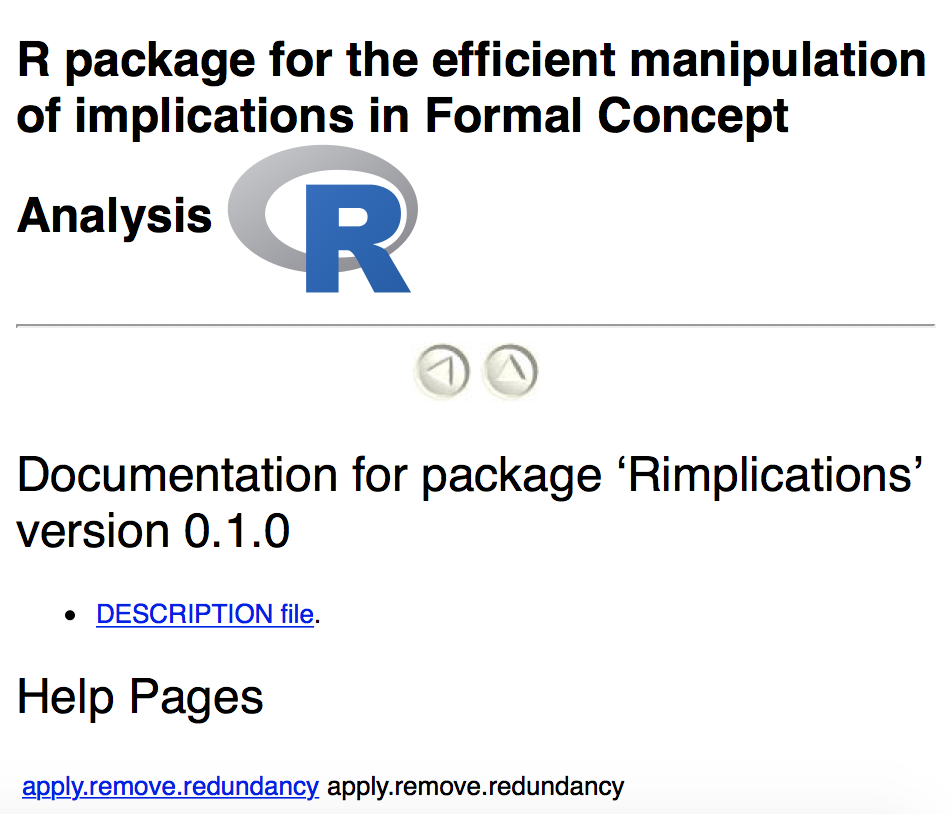
\includegraphics[scale=0.6]{docs2}
    \caption{Ejemplo Documentaci\'on 2}
    \label{fig:docs2}
\end{figure}

Aqu\'i se ve la documentaci\'on del algoritmo para la eliminaci\'on de redundancia:
\begin{figure}[H]
    \centering
    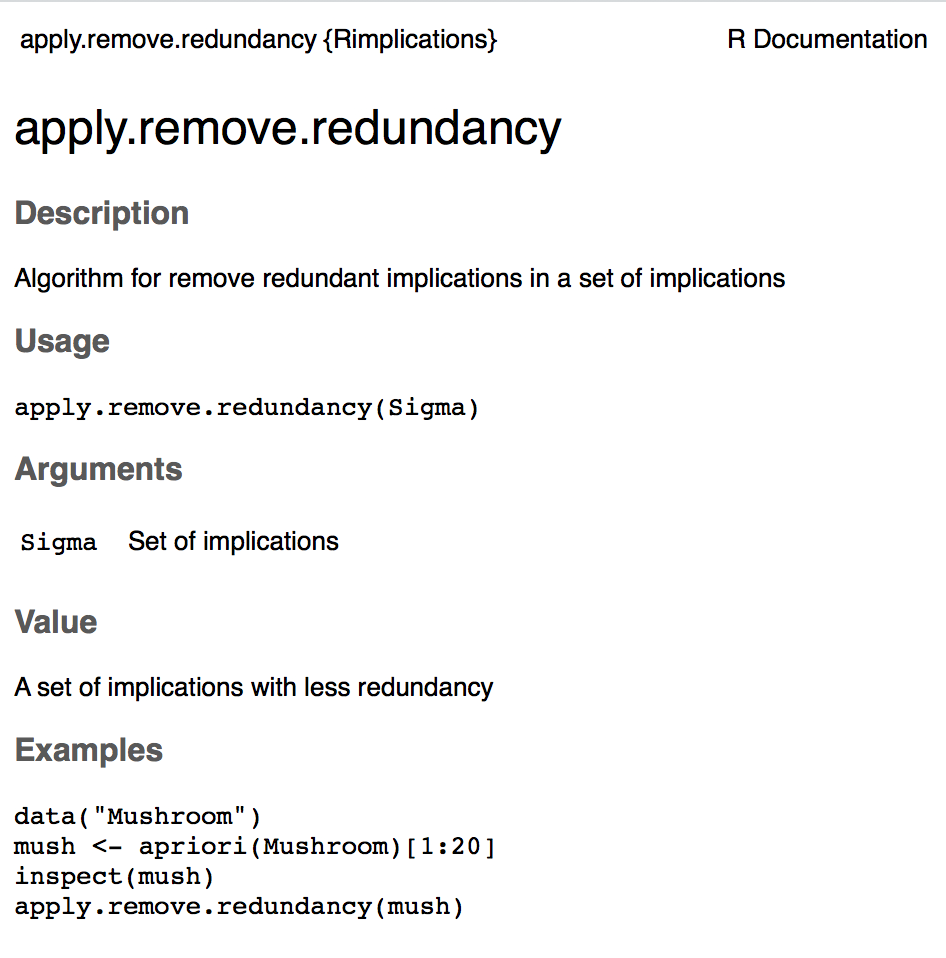
\includegraphics[scale=0.75]{docs3}
    \caption{Ejemplo Documentaci\'on 3}
    \label{fig:docs3}
\end{figure}
\newpage

\end{document}